\documentclass[11pt,a4paper]{scrbook}

%---------- Packages ----------
\usepackage[latin1]{inputenc}
\usepackage{xspace}
\usepackage{hyperref}
\usepackage{booktabs}
\usepackage{listings}
\usepackage{graphicx}
\usepackage{subfig}
\usepackage{tikz}
\usepackage{geometry}
\usepackage{fancyhdr}

\newcommand{\libalf}{\texttt{libALF}\xspace}
\newcommand{\cpp}{C+$\!$+\xspace}
\newcommand{\java}{\texttt{Java}\xspace}
\newcommand{\offline}{\emph{offline}\xspace}
\newcommand{\online}{\emph{online}\xspace}
\newcommand{\teacher}{\emph{teacher}\xspace}
\newcommand{\alphsize}{\emph{alphabet size}\xspace}
\newcommand{\conjecture}{\texttt{conjecture}\xspace}
\newcommand{\cj}{\texttt{cj}\xspace}
\newcommand{\advanced}{\emph{advance}\xspace}
\newcommand{\memque}{\emph{membership queries}\xspace}
\newcommand{\accepted}{\emph{accepted}\xspace}
\newcommand{\rejected}{\emph{rejected}\xspace}
\newcommand{\result}{\texttt{result}\xspace}
\newcommand{\stringtype}{\texttt{String}\xspace}
\newcommand{\inputs}{\texttt{input}\xspace}
\newcommand{\checkeq}{\texttt{check\_equivalence\(\)}\xspace}
\newcommand{\answer}{\texttt{answerMembership}\xspace}
\newcommand{\getqueries}{\texttt{get\_queries\(\)}\xspace}
\newcommand{\getsize}{\texttt{get\_alphabetsize\(\)}\xspace}
\newcommand{\filters}{\emph{filters}\xspace}
\newcommand{\normalizers}{\emph{normalizers}\xspace}
\newcommand{\vectored}{\texttt{vector}\xspace}
\newcommand{\node}{\texttt{node}\xspace}
\newcommand{\integer}{\texttt{integer}\xspace}
\newcommand{\true}{\texttt{true}\xspace}
\newcommand{\false}{\texttt{false}\xspace}


%---------- Make index ----------
\makeindex

%---------- Title & Author ----------
\title{The \texttt{libalf} Library}

%---------- Document begins ----------
\begin{document}

%---------- fancy headings ----------
\pagestyle{fancy}


%---------- Title ----------
\maketitle{}


%---------- Table of Contents ----------
\tableofcontents
\listoffigures
\listoftables
\cleardoublepage

%---------- Content ----------

\chapter{Introduction}

\section{\libalf Basics}
		The \libalf library is an actively developed, stable, and extensively-tested library for learning finite state machines. It unifies different kinds of learning techniques into a single flexible, easy-to-extend, open source library with a clear and easy-to-understand user interface.
		\paragraph{}	
		The \libalf Library provides a wide range of \online and \offline algorithms for learning Deterministic (DFA) and Nondeterministic Finite Automata (NFA). \online algorithm is a technique where the hypothesis is built by understanding the classification (whether accepted or rejected) of queries asked to some kind of a \teacher.  While, an \offline algorithm builds an apposite hypothesis from a set of classified examples that were passively provided to it. As of \today, the library contains seven such algorithms implemented in it which are listed in Table \ref{algtables}.

		\begin{table}
		\centering
		\begin{tabular}[c]{lcr}
		\toprule[1pt]
			Online Algorithms & Offline Algorithms \\	
		\midrule
			Angluin's L [2] (two variants) & Biermann [3] \\
			NL [4] & RPNI [13] \\
			Kearns / Vazirani [10] & DeLeTe2 [6]\\
		\bottomrule[1pt]
		\end{tabular}
		\caption{List of Algorithms Implemented}
		\label{algtables}
		\end{table}
		
	  \paragraph{}	
		The central aim of \libalf Library is to provide significant advantages through potential features to the user. Our design of the tool primarily focuses on offering high flexibility and extensibility. 
	  \paragraph{}	
		Flexibility is realized through two essential features the library offers. The first being the support for switching easily between learning algorithms and information sources, which allows the user to experiment with different learning techniques. The second being the versatility of the tool. Since it is available in both \cpp and \java (using the Java Native Interface), it can be used in all familiar operating systems (Windows, Linux and MacOS in 32- and 64-bit). In addition, the dispatcher implements a network based client-server architecture, which allows one to run \libalf not only in local environment but also remotely, e.g., on a high performance machine.
		\paragraph{}
		In contrast, the goal of extensibility is to provide easy means to augment the library. This is mainly achieved by \libalf's easy-to-extend design and distributing \libalf freely as open source code. Its modular design and its implementation in \cpp makes it the ideal platform for adding and engineering further, other efficient learning algorithms for new target models (e.g., B?chi automata, timed automata, or probabilistic automata). 
		\paragraph{}
		Other pivotal features of the library include, ability to change the \alphsize during the learning process, extensive logging facilities, domain-based optimizations via so-called normalizers and filters, GraphViz visualization.
		
		
\section{Conceptual Details}

	The \libalf consists of four main components, the Learning Algorithm, the Knowledgebase, Filters \& Normalizers and Logger \& Statistics. Figure \ref{fig:components} shows a characteristic view of the these components. Our implementation of these components allows for plug and play usage.

\begin{figure}[h]
  \centering
  \subfloat[Algorithms]{\label{fig:alg}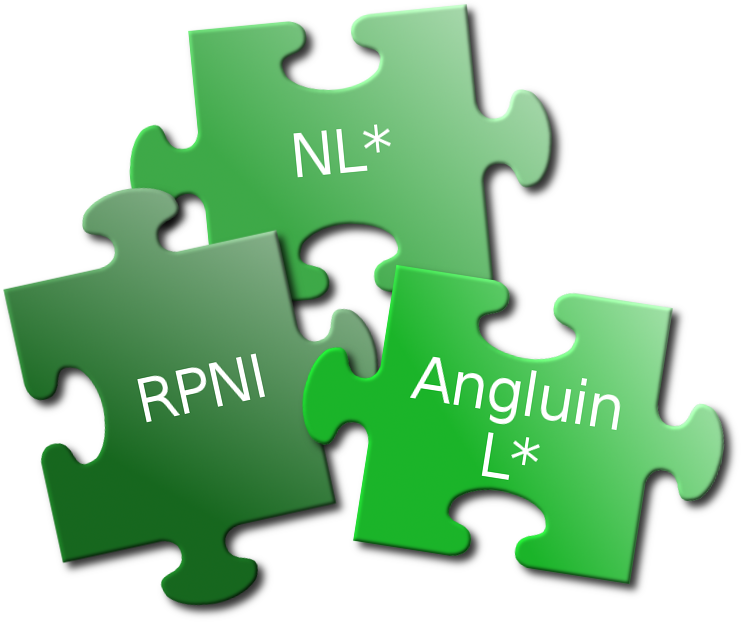
\includegraphics[width=0.35\textwidth,scale=0.3]{Images/1.png}}  \hspace{30pt}           
  \subfloat[Knowledgebase]{\label{fig:base}
\includegraphics[width=0.3\textwidth]{Images/2.png}}\\
  \subfloat[Filter \& Normalizer]{\label{fig:filter}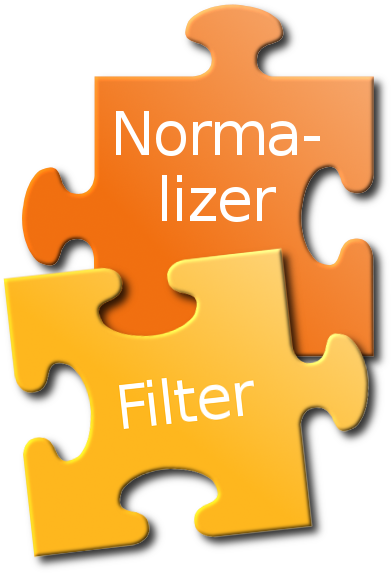
\includegraphics[width=0.27\textwidth]{Images/3.png}} \hspace{30pt}
  \subfloat[Logger \& Statistics]{\label{fig:logger}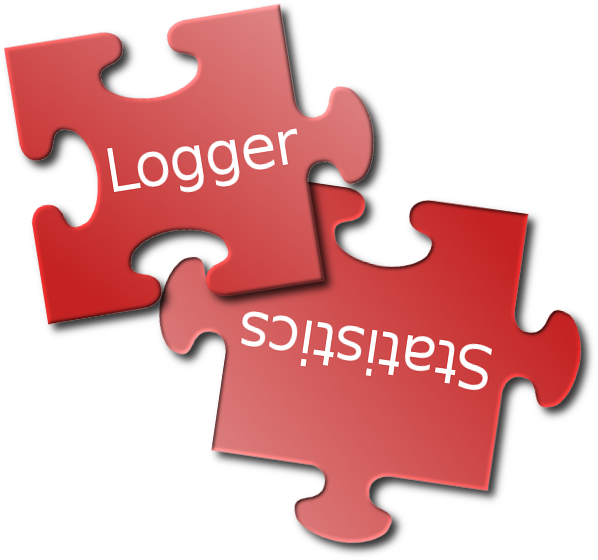
\includegraphics[width=0.35\textwidth]{Images/4.png}}
  \caption{Components of \libalf}
  \label{fig:components}
\end{figure} 
	
\subsection{The Knowledgebase}

	The knowledgebase is an efficient storage for language information that accumulates every word and its associated classification. It allows storage of values of arbitrary types and in the forthcoming sections we will describe its implementation where a word is stored as a list or array of \texttt{Integers}.
	It forms the fundamental source of information for a learning algorithm. Using an external storage for the knowledgebase has the advantage of it being independent of the choice of the learning algorithm. This enables interchanging of learning algorithms on the basis of same knowledge available. 
	
\begin{figure}[h]
	\centering
	\subfloat{\label{fig:baseandalg}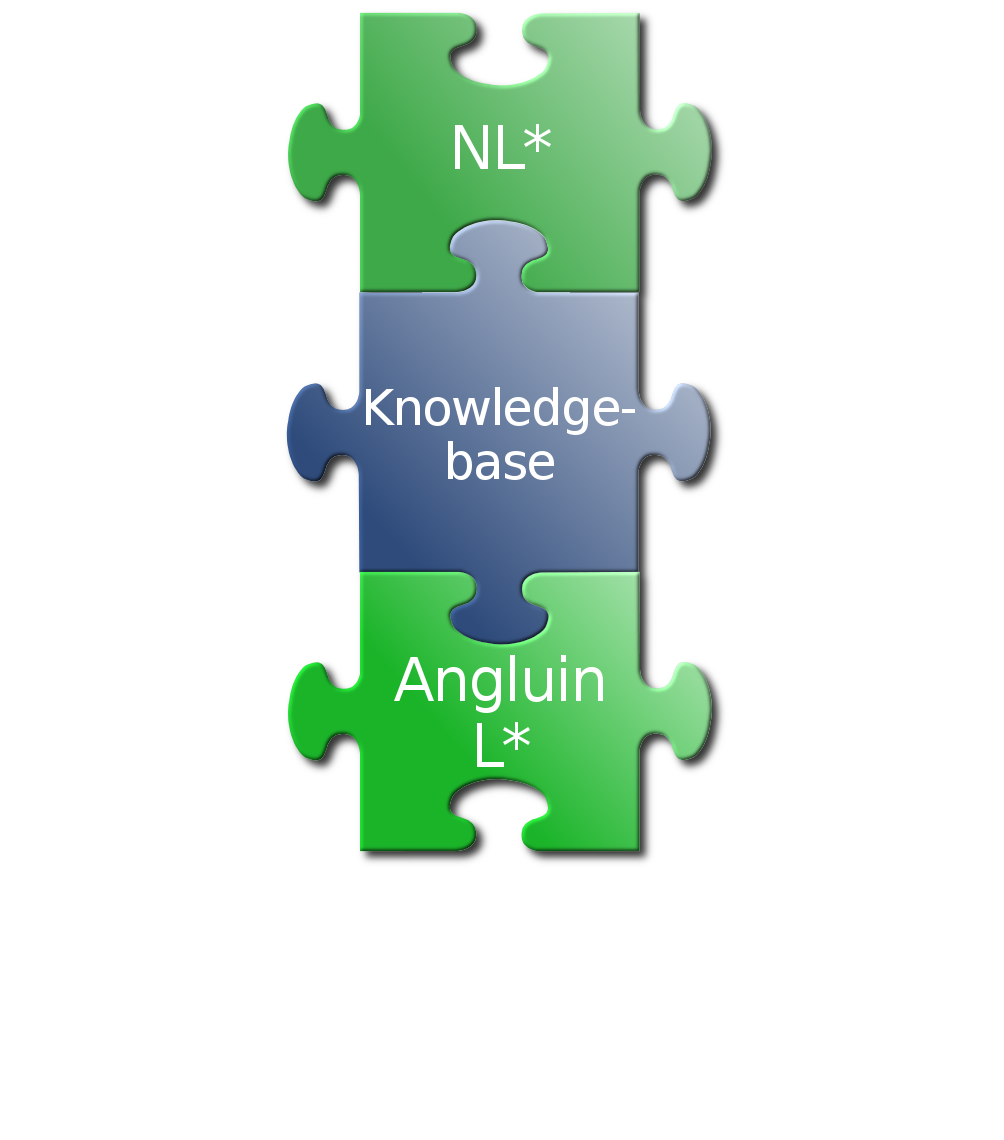
\includegraphics[width=0.5\textwidth]{Images/combined3.png}}
	\subfloat{\label{fig:basealgfilt}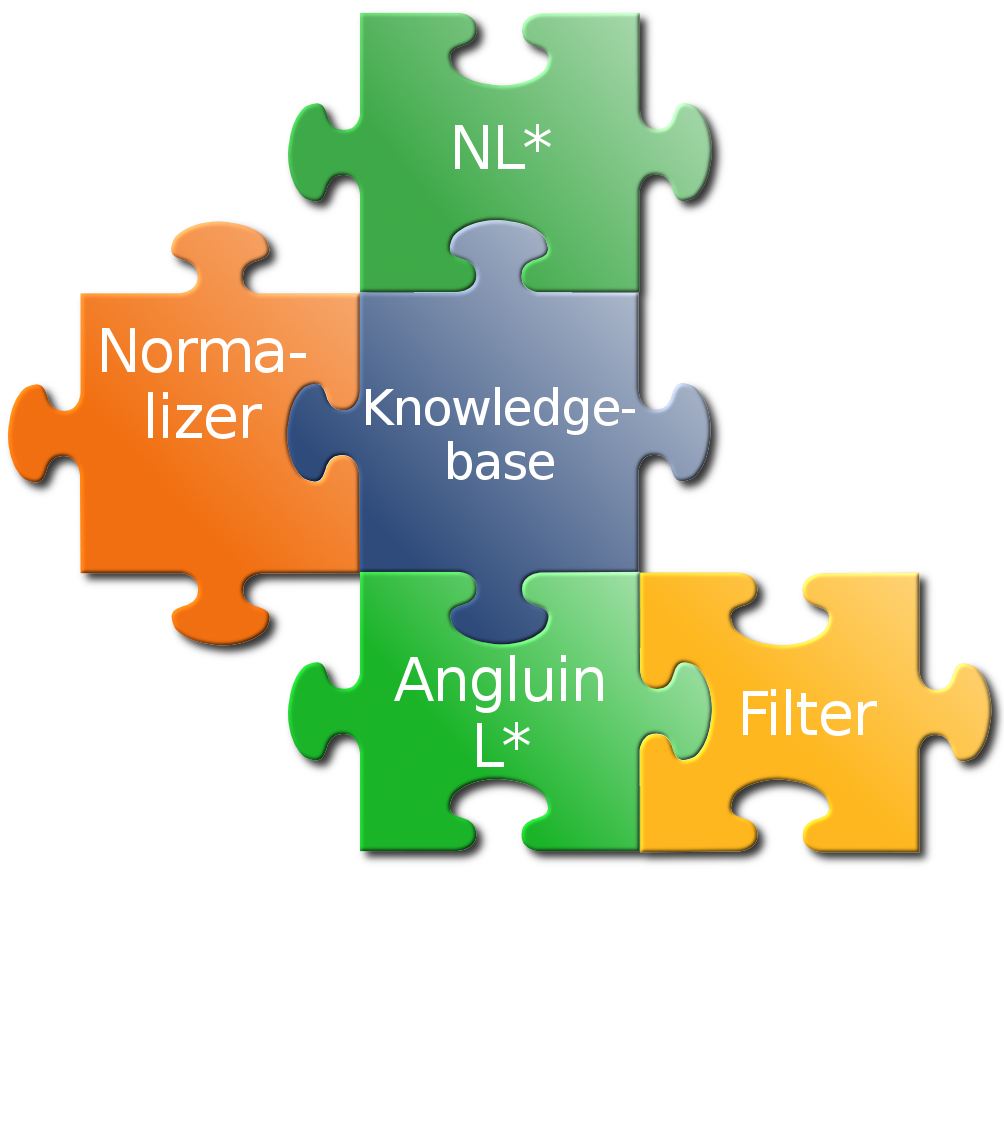
\includegraphics[width=0.5\textwidth]{Images/combined5.png}}
	\caption{Pictorial Representation of Plug and Play support}
	\label{fig:plug}
\end{figure}

\subsection{Learning Algorithm}
	A learning algorithm is a component that retrieves the desired information from the knowledgebase to construct a conjecture. As mentioned in the previous section, there exists two types of learning algorithms - \offline and \online algorithm. 
	\paragraph{}
	The workflow of the algorithms begins with a common step wherein the algorithm is supplied with information about size of the alphabet for the conjecture. Thereafter, the algorithms follow two separate procedures to compute the conjecture.
	
	The \offline algorithm continues as stated below.
\begin{enumerate}
	\item The knowledgebase is furnished with the set of words and their classifications (provided by the user).
	\item When all details have been supplied and is available in the knowledgebase, the learning algorithm is made to advance to 	compute the conjecture in conformance with the samples.
\end{enumerate}

	An \online algorithm proceeds in the following manner. \\
	The following two steps are repeated until a correct conjecture is determined.
\begin{enumerate}
\item The algorithm is made to advance.
\item Here one of the following two possible events may occur.
\begin{enumerate}
\item If no hypothesis is created, ``membership queries'' that require associated classification are resolved (by the \teacher) and added to the knowledgebase.
\item If a hypothesis was created, the ``equivalence query'' is answered by the teacher. If the conjecture is incorrect a counter example is rendered by the teacher.
\end{enumerate}
\end{enumerate}	
	
An insight into the working of the two algorithms is given in Section 1.3.
	
\subsection{Filters and Normalizers}	
	The knowledgebase can be associated with a number of \filters, which are used for domain-specific optimization. This implies that the knowledgebase makes use of domain-specific information to reduce the number of queries to the teacher. Such filters can be composed by logical connectors (and, or, not). In contrast, \normalizers are able to recognize words equivalent in a domain-specific sense to reduce the amount of knowledge that has to be stored. 
		
\subsection{Loggers and Statistics}	
	The library additionally features means for statistical evaluation or loggers. A logger is an adjustable logging facility that an algorithm can write to, to ease application debugging and development. The modularity of our approach in developing \libalf facilitates these components to be added in an easy plug and play fashion and that is shown in Figure \ref{fig:plug} and Figure \ref{fig:loggers}.
	
\begin{figure}[h]
	\centering
	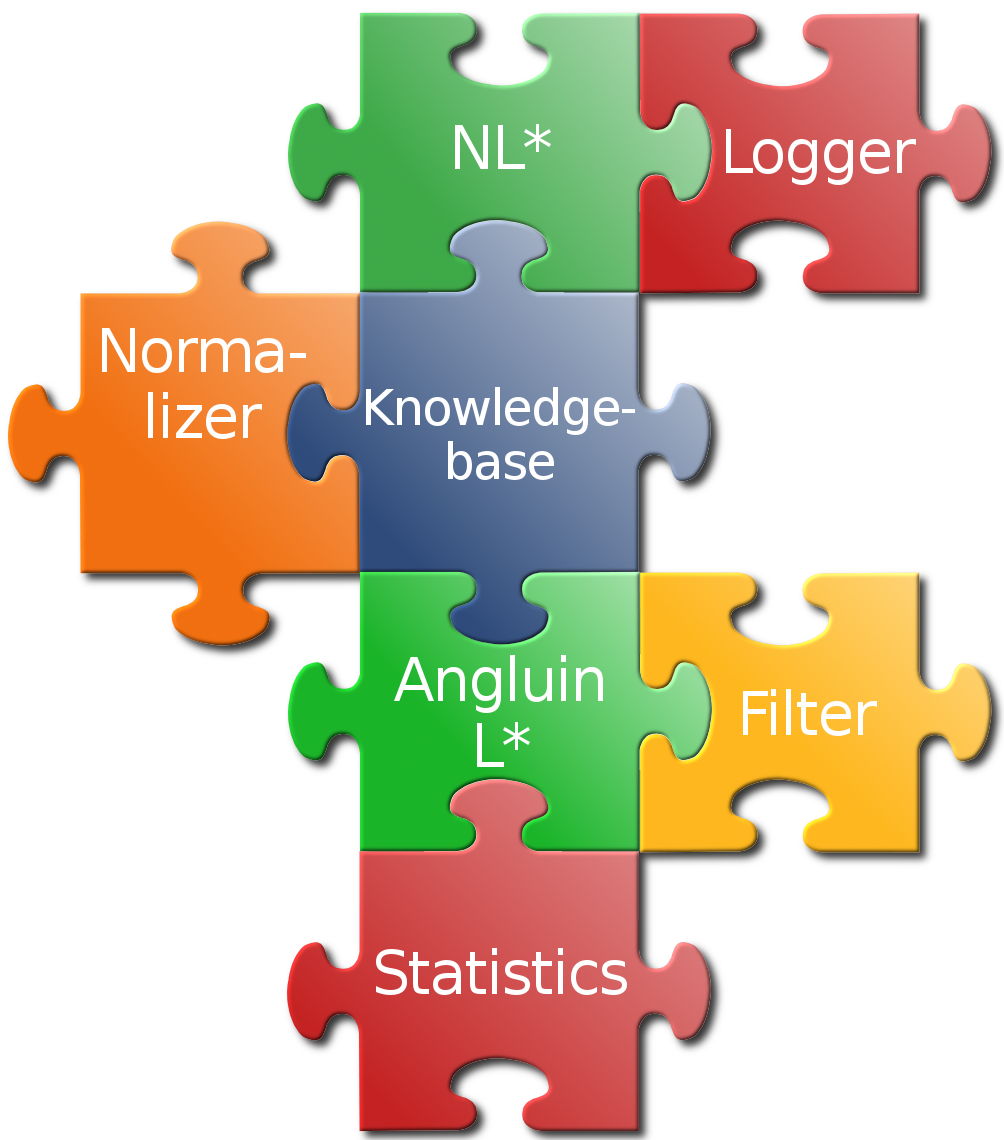
\includegraphics[width=0.5\textwidth]{Images/combined6.png}
	\caption{Addition of Loggers and Statistics in Plug and Play fashion}
	\label{fig:loggers}
\end{figure}
	
\subsection{Connections of the Components}

The primary aspect in describing the working would be to outline the data flow between a learning algorithm, the knowledgebase and the user (or \emph{teacher}) as sketched in Figure \ref{communications}.

\begin{figure}
\centering
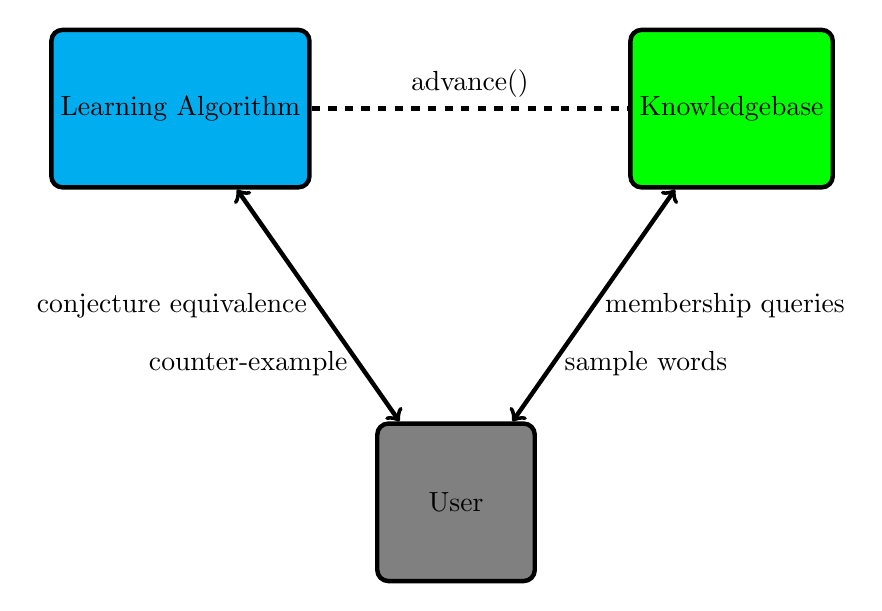
\begin{tikzpicture}[rounded corners,ultra thick]
\draw node[minimum height=2cm,minimum width=2cm,fill=cyan,draw] (la) at (0,5) {Learning Algorithm};
\draw node[minimum height=2cm,minimum width=2cm,fill=green,draw] (kn) at (7,5) {Knowledgebase};
\draw node[minimum height=2cm,minimum width=2cm,fill=gray,draw] (user) at (3.5,0) {User};
\draw[dashed,ultra thick] (la) -- (kn) node[midway,above] {advance()};
\draw[<->,ultra thick] (la) -- (user) node[midway,left] {conjecture equivalence} node[near end,left] {counter-example};
\draw[<->,ultra thick] (kn) -- (user) node[midway,right] {membership queries} node[near end,right] {sample words};
\end{tikzpicture}
\caption{data flow of the \libalf components}
\label{communications}
\end{figure}

The learning algorithm and the knowledgebase share information with user. The knowledgebase, as stated earlier, is the fundamental information for the learning algorithm to develop an automaton. The learning algorithm advances with whatever knowledge is available. The learning algorithm connects with the user to collect relevant information such as equivalence of a conjecture or to retrieve counter-example. When the learning algorithm creates more membership queries, they are stored in the knowledgebase leading to it initiating a communication with the user who is required to answer membership queries (or input sample words in case of an offline algorithm). All such information extended by the user are stored in the knowledgebase. 

\section{Demo Application}

In this section we describe the working of the \offline and \online algorithms with reference to the demo code in \cpp available at our website \url{http://libalf.informatik.rwth-aachen.de/}. Demo programs of the algorithms in \java are also available there.

The following code snippet briefly demonstrates how to employ the \libalf library in a user application. It is important that you become familiar with the auxilliary methods used in the program and hence their operations are explained first.

\begin{itemize}
\item \textbf{\emph{get\_AlphabetSize()}} - Prompts the user to provide information about the size of alphabet and stores it as an \texttt{Integer}.
\item \textbf{\emph{answer\_Membership(\*li)}} - Takes the list of queries as an argument and presents it to the user to classify them. It returns \texttt{true} when the word is to be accepted and returns \texttt{false} when it is to be rejected.
\item \textbf{\emph{check\_Equivalence(cj)}} - Presents the computed conjecture to the user who marks it as correct or incorrect. Returns \texttt{true} or \texttt{false} respectively.
\item \textbf{\emph{get\_CounterExample(alphabetsize)}} - Requests the user to input the counter-example and returns the word as a list (array in \java implementation) of integers. It takes the alphabetsize as a parameter for validation purposes.
\item \textbf{\emph{get\_Samples(alphabetsize)}} - Retrieves the sample word from the user. The alphabetsize is passed as a parameter for validation purposes.
\item \textbf{\emph{classification = get\_Classification()}} - Retrieves the classification of the sample word from the user. Returns \texttt{true} when the word is to be accepted and returns \texttt{false} when it is to be rejected.
\item \textbf{\emph{enough\_Samples()}} - Requests the user to specify whether all samples have been provided by the user. Returns ``y'' if user desires addition of more samples or ``n'' if all samples have been provided already.
\end{itemize}

\subsection{Online Algorithm}

An \online Algorithm, as mentioned in the previous section, formulates the conjecture by putting forth ``queries'' to the \teacher.

\lstset{language=c++, numbers=left, numberstyle=\tiny, stepnumber=1, numbersep=5pt}
\begin{lstlisting}[frame=single]
void main(int argc, char**argv) {
int alphabetsize = get_AlphabetSize();
knowledgebase<bool> base;
angluin_simple_table<bool> algorithm(&base,
NULL,alphabetsize);
do {
 conjecture * cj = algorithm.advance();
 if (cj == NULL) 
 {
   list<list<int> > queries = base.get_queries();
   list<list<int> >::iterator li;
   for(li = queries.begin(); li != queries.end(); li++) 
   {
      bool a = answer_Membership(*li);
      base.add_knowledge(*li, a);
   }
 }
 else 
 {
   bool is_equivalent = check_Equivalence(cj);
   if (is_equivalent) result = cj; 
   else 
   {	
      list<int> ce = get_CounterExample(alphabetsize);
      algorithm.add_counterexample(ce);
   }
 }
}while (result == NULL);
cout<<result->visualize();
}
\end{lstlisting}

The workflow of the program is as described below:

\begin{enumerate}
	\item At line 2, the program prompts the user to input the \alphsize of the Automaton.
	\item An empty knowledgebase is now initialized at line 3. (The knowledgebase stores the words as a list of \texttt{Integers})
	\item Now, a learning algorithm is created by providing three parameters - the knowledgebase, NULL for a logger, the Alphabet Size.
	\item After having initialized the learning algorithm, the program is subjected to a loop where the algorithm is made to \advanced (Line 7). The result of this is stored in a \conjecture type variable \cj.
	
	\item If there was no sufficient information available in the knowledgebase to construct a conjecture, then \cj is NULL and the algorithm enters the condition at line 8. The algorithm produces the \memque that needs to be resolved by the user (or \teacher). The queries are obtained using the method \getqueries. (Note: the queries are obtained in ``list of list of \texttt{Integers}'' since words are stored as \texttt{Integers} and there may be more than one query)
	
	\item The queries produced are presented to the user who classifies it as \accepted or \rejected. This is done at Line 13 with \answer function. Subsequently, This information is added to the knowledgebase and the iteration of the loop continues.

	\item However, if a conjecture was computed at line 7, (implying that enough information was available in the knowledgebase), then algorithm enters the condition at line 18. The conjecture is presented to the user by \checkeq function at line 20.
	
	\item If the conjecture is equivalent, the user marks it correct and the conjecture is stored in variable \result. Iteration ends and the \result is displayed in line 32.
	
	\item If it is not equivalent, the user is now prompted to provide a counter example (line 27) and the program continues with the iteration. Typically, the counter example would influence the learning algorithm to invoke more \memque that is to be resolved during the next \advanced of the algorithm.
\end{enumerate}

\subsection{Offline Algorithm}

An \offline algorithm, as mentioned in the previous section, computes a conjecture from a set of passively provided input samples with their classifications.

\lstset{language=c++, numbers=left, numberstyle=\tiny, stepnumber=1, numbersep=5pt}
\begin{lstlisting}[frame=single]
int main(int argc, char**argv) 
{
  int alphabetsize = get_AlphabetSize();
  string input = "y";
  list<int> words;
  bool classification;
  knowledgebase<bool> base; 
  while (input == "y") 
  {
    words = get_Samples(alphabetsize);
    classification = get_Classification();
    base.add_knowledge(words, classification);
    input = enough_Samples();
  }
  RPNI<bool> algorithm(&base, NULL, alphabetsize);
  conjecture *cj = algorithm.advance();
  cout <<cj->visualize();
}
\end{lstlisting}

The workflow of the above program is as follows:

\begin{enumerate}

\item At line 2, the program prompts the user to input the \alphsize used for the automaton (coded in the function \getsize)
\item Variables for storing the sample words and their classifications are described subsequently. An empty knowledgebase is now initialized. 
\item The program then passes over a loop which recursively performs the action of reading the sample (line 10) and its classification (line 11) from the user. As and when the user inputs this information, it is continually added to the knowledgebase (line 13). The loop ends when the user indicates that the desired number of samples have been entered as coded in line 13 (its for this purpose that the \stringtype \inputs is first initialized to ``y'').
\item Now, a learning algorithm (RPNI Offline Algorithm) is created by providing three parameters - the knowledgebase, NULL for a logger, the Alphabet Size (line 15)
\item Having initialized the algorithm, it is now made to \advanced which produces a conjecture that pertains to the user's specification of samples. (line 16)
\item Finally, the conjecture is printed as coded in line 17 of the program.

\end{enumerate}

In both the command line programs implemented in \cpp and \java, the program outputs the ``.dot'' file which contains the code that builds the conjecture graphically. (This file may be executed using the GraphVIZ tool).



\chapter{Compiling and Installing \libalf}
This chapter will guide you through the compilation and installation of \libalf on Linux and Windows. 

\libalf works on Linux and Windows on both 32- and 64-bit architectures. However, as \libalf has no prerequisites, it is most likely that it also runs on various additional operating systems. If you want to compile \libalf for another operating system, e.g.\ MacOS X, the guidelines for compiling \libalf for Linux may be a good reference. 

This document is organized in six sections: The first two sections describe how to obtain \libalf (if you not already have) and what prerequisites need to be fulfilled. Sections \ref{sec:install_libalf} to \ref{sec:install_dispatcher} show how to compile and use \libalf, \jalf and dispatcher. The sixth section gives help on troubleshooting.

%---------- Libalf Package Information -----------
\section{\libalf Package Information}\label{sec:install_package_info}
The library is freely available under the open source LGPL v3 license at the \libalf website \url{http://libalf.informatik.rwth-aachen.de}. Download the \libalf package and extract it to a folder of your choice. The package contains the following components:
\begin{itemize}
  \item The \libalf \cpp library.
  \item \jalf (\libalf's Java interface).
  \item The dispatcher (a network-based \libalf server).
\end{itemize}

This guide will demonstrate how to employ and use \libalf in user applications through \emph{examples} available at \libalf's website. We recommend that you download and extract the example sources to a folder of your choice.

\section{Prerequisites}
The \libalf library itself does not have any prerequisites, but some components have. To use the additional components, please ensure that the following requirements are satisfied.

\begin{itemize}
  \item For compiling and using \jalf you need a Java Development Kit (JDK) Version 6.0 or later installed. Moreover, we recommend using the \emph{Ant} build tool downloadable from \url{http://ant.apache.org/}.
  \item The dispatcher requires a POSIX-compliant operating system. While there is no problem under Linux, the dispatcher will not compile under Windows.
\end{itemize}

\paragraph{Linux.}
For compiling the \cpp sources in Linux, you require a \cpp compiler (this document assumes that you use the \emph{GNU \cpp compiler}) and the \emph{make utility}, which is used to automate the build process. Both tools should be installed by default on every Linux machine.

\paragraph{Windows.}
To compile the \cpp sources on Windows, we recommend using the \emph{Minimalist GNU for Windows (MinGW)} compiler and \emph{MSYS}, a Unix-style shell for Windows. Both can be obtained from \url{http://www.mingw.org/}. 

Please follow the instructions on the website to set up MinGW and MSYS properly. In particular, make sure that you install the MSYS make package (if not done automatically). Using MSYS gives you the advantage of following all instructions described in this document no matter whether you use Linux or Windows. However, please be careful with folder names that contain blanks; you may have to enclose them in quotes and replace every blank with a backslash followed by a blank (or, in the best case, you avoid them completely).

%---------- The libALF C++ Library -----------
\section{\texorpdfstring{The \libalf \cpp Library}{The \libalf C++ Library}}\label{sec:install_libalf}
The section will describe how to compile and install the library as well as how to run applications that use the library.

\subsection{Compiling \libalf}
You have the choice to compile the \libalf library either as a \emph{static} or as a \emph{shared} library. If you do not know the difference or if you just want to use the library, you should compile a shared library as described below and follow the respective instructions for running your application.

\subsection*{Compiling a Shared Library}
Compiling \libalf is easy: simply change into the \texttt{libalf/src} folder and invoke the make utility by typing 

\cmd{make} 

The make utility automatically detects which operating system you are running and compiles the library accordingly. After the compilation you should find the binary file \texttt{libalf.so} (on Linux) or \texttt{libalf.dll} (on Windows) inside the \texttt{libalf/src} folder. However, if you experience problems, you can explicitly tell the make utility for which system you want to compile \libalf by typing \texttt{make libalf.so} (under Linux) or \texttt{make libalf.dll} (under Windows).

\subsection*{Compiling a Static Library}
You can compile a static library using the command (inside \texttt{libalf/src})

\cmd{make libalf.a}

on both Linux and Windows.

However, make sure that you delete any shared library in the folder before you link your application with libalf as some operating systems (e.g. Linux) always prefer shared libraries if present.

\subsection{Installing \libalf}
Installing \libalf means to copy to the compiled shared library and \libalf's headers to a location where your operating system finds them.

\paragraph{Linux.}
To install \libalf in Linux, first compile the library and type \texttt{make install}. You can uninstall \libalf by using the command \texttt{make uninstall}. Please note that you need root privileges for both actions.

\paragraph{Windows.}
On Windows, you have to manually copy the compiled shared binary files to your \texttt{windows/system} directory. Unfortunately, there is no common place to put header files in. Thus, you have to specify the header's location every time you compile an application that uses \libalf (see the section below).

\subsection{Compiling Applications That Use \libalf}
When compiling an application that uses \libalf, the compiler needs to find \libalf's headers and the compiled library. Please note that you do not have to provide this information if you have libalf installed on your system.

Otherwise, you have to use the GNU C++ compiler's \texttt{-I} parameter to specify \libalf's header locations (typically \texttt{libalf/include}) and the \texttt{-L} parameter to specify the location for the compiled library (which is \texttt{libalf/src}). You also have to link the application to \libalf using \texttt{-lalf}.

We will consider the online-example to explain the compilation.

\paragraph{Compiling applications that links to shared library.}
To compile the online example that uses the shared library, type the following command.

\cmd{g++ -I path\_to\_headers -L path\_to\_library online.cpp -lalf}

\paragraph{Compiling applications that links to static library.}
If you want to link libalf statically into your application, you can do so by adding \texttt{-static} as additional parameter just before linking to libalf like below.

\cmd{g++ -I path\_to\_headers -L path\_to\_library online.cpp -static -lalf}
\paragraph{}
In both cases, it is also a good idea to specify the name of the output file using the \texttt{-o} parameter, e.g. \texttt{-o online}.

\paragraph{Additional Parameter for Windows.}
Please note that on Windows the Winsock2 library has to be linked additionally to every program using \libalf. You can do this by adding \texttt{-lws2\_32}. Again it is crucial that you add this parameter after all input files.

\subsection{Running Applications That Use \libalf}
An application \emph{statically} linked to libalf can be executed as usual. However, if you run a program that uses \libalf as a \emph{shared library}, you need to specify where your operating system can find the library (again, you do not need to provide this information if you have installed \libalf on your system).

\paragraph{Linux.}
On Linux, use the \texttt{LD\_LIBRARY\_PATH} variable to point to the location of the shared library. For instance, you can run the above compiled online example with the command

\cmd{LD\_LIBRARY\_PATH=path\_to\_library ./online}

\paragraph{Windows.}
Unfortunately, on Windows there is no direct way of telling the system where to find shared libraries. Instead, you have to add their locations to Windows' \texttt{PATH} variable or copy the library into the folder your application is executed from. Then, execute your application as usual.

For further details please refer to the examples' Readme and Makefile.

%---------- The jalf Java Library -----------
\section{\texorpdfstring{The \jalf Java Library}{The jALF Java Library}}\label{sec:install_jalf}
\jalf is the Java interface to \libalf. It lets you access \libalf via the dispatcher or via Java's \emph{Native Inter-face JNI}. The latter way requires that you compile a second \cpp library (some kind of wrapper), that obeys Java's naming convention and performs some basic conversions of internal data structures. However, if you want to use \jalf only in connection with the dispatcher, it is enough to compile and use the Java sources.

In the following we assume that you are familiar with basics of compiling and running Java programs.

\subsection{Compiling \jalf's Java sources}
In order to compile \jalf's Java sources, change to the \texttt{libalf/jalf} folder and type

\cmd{ant}
\paragraph{}
This invokes the Ant build utility and produces the file \texttt{jalf.jar} containing all compiled class files inside the \texttt{libalf/jalf} folder. If you do not wish to use \jalf via JNI, you can skip compiling \jalf's \cpp sources.

Note that you can generate \jalf's \emph{JavaDoc} also using Ant with the command \texttt{ant doc}. Thereafter, the JavaDoc can be found inside the \texttt{libalf/jalf/java/doc} folder.

\subsection{\texorpdfstring{Compiling \jalf's \cpp Sources}{Compiling jALF's C++ Sources}}
The \jalf \cpp library needs to be a shared library. However, you have the option to link \libalf either dynamically or statically to \jalf. The latter option is often preferred and enabled by default. Please remember to delete any shared library in \texttt{libalf/src} before you compile \jalf's \cpp sources (\libalf is recompiled for you). You may use the command \texttt{make -C libalf/src clean} for this.

Compiling \jalf's \cpp sources is also automated by means of the make utility. However, as additional information the Java compiler requires the location of Java's JNI header files, which are contained in every JDK. Their location is passed on to the make utility using the \texttt{JAVA\_INCLUDE} variable. Thus, to compile \jalf's \cpp sources, go to \texttt{libalf/jalf/src} and execute

\cmd{JAVA\_INCLUDE=path\_to\_jdk/include make}

\paragraph{}
Again, the make utility should detect your operating system automatically, but you can also use the commands \texttt{make libjalf.so} (for Linux) and \texttt{make jalf.dll} (for Windows) to explicitly compile \jalf for your desired operating system. After a successful compilation, the compiled binary is located in \texttt{libalf/jalf/src}.

\paragraph{Dynamic Linking.}
As mentioned, \libalf is linked statically by default. If you want link \libalf \emph{dynamically}, you can use the commands \texttt{make libjalf.so-dynamic} (for Linux) and \texttt{make jalf.dll-dynamic} (for Windows).

\subsection{Compiling Java applications that use \jalf}
Fortunately, the Java compiler does not need to know anything about the \cpp libraries to compile your application and only needs access to \jalf's Java class files. You specify this information by adding the \texttt{jalf.jar} file to Java's classpath. Our Java online example, for instance, can be compiled using the following command (first change into the folder containing the example sources):

\cmd{javac -classpath "path\_to\_jalf/jalf.jar" Online.java}

\subsection{Running Java applications that use \jalf}
Besides the location of the \texttt{jalf.jar}, running a Java application that uses \jalf requires telling Java where it can find the compiled \jalf and \libalf \cpp libraries. (If you have installed \libalf to your system or if you linked \jalf statically to \jalf, you do not need to bother about the latter.)

The place where Java looks for \cpp libraries is controlled by Java's interval library path variable. This variable can only be changed at the start of the Java VM. You do so by setting the variable named \texttt{java.library.path} to the location of the \jalf library (i.e, the \jalf \cpp binary which is typically \texttt{libalf/jalf/src}) using the \texttt{-D} parameter. 

\paragraph{Linux.}
To run the online example on Linux, one has to execute the following command (inside the folder containing the compiled online example):

\cmd{java -classpath "path\_to\_jalf/jalf.jar:." \\\phantom{java }-Djava.library.path=path\_to\_jalf\_library Online}

If necessary, specify the location of the shared \libalf library as described in Section \ref{sec:install_libalf}.

\paragraph{Windows.}
Please recall that Linux and Windows use different ways of separating folders. While you must use a colon on Linux, you must use a semicolon on Windows; everything else is the same as before.

\cmd{java -classpath "path\_to\_jalf/jalf.jar;." \\\phantom{java }-Djava.library.path=path\_to\_jalf\_library Online}

\paragraph{}
For further details please refer to the examples' Readme.

%---------- Compiling and Using the Dispatcher ----------
\section{Compiling and Using the Dispatcher}\label{sec:install_dispatcher}
Please recall that the dispatcher only compiles and runs on a POSIX-compliant operating system such as Linux, but not on Windows.

\subsection{Compiling the Dispatcher}
To compile the dispatcher, first compile a shared \libalf library as described Section \ref{sec:install_libalf}.

\paragraph{Dynamic Linking.}
By default, the dispatcher is dynamically linked to \libalf. To compile an executable linked statically, change into the folder \texttt{libalf/dispatcher} and execute

\cmd{make}

This creates the executable dispatcher in the same directory. 

\paragraph{Static Linking.}
To link the dispatcher statically to \libalf, use the following command

\cmd{make dispatcher-static}

Again, remember to remove any compiled shared library in \texttt{libalf/src} first.

\subsection{Running the Dispatcher}
The dispatcher is executed like any other executable on your system. However, remember to specify the location of the \libalf shared library if necessary.


%---------- Troubleshooting ----------
\section{Troubleshooting}


When experiencing troubles, the first thing you should try is to execute \texttt{make clean} in the \texttt{libalf} and \texttt{libalf/jalf} folders as well as \texttt{ant clean} in the \texttt{libalf/jalf} folder. This deletes all compiled files and solves most compiler and linker problems. However, if this does not work for you, you may find a solution for your problem in the list below:

\begin{itemize}
  \item There are no known problems.
\end{itemize}

\chapter{The Knowledgebase}

The knowledgebase is the central repository of membership information. It is a database that stores words and their classifications. Apart from this basic functionality, the knowledgebase also offers number of other features thereby increasing the support for extensibility.
These features are reflected in its implementation wherein the methods used in the knowledgebase can be divided into two categories - \textbf{\emph{Methods important for Using \libalf}} and \textbf{\emph{Methods important for expanding \libalf}}. 
\paragraph{}
The chapter discusses these methods from both a user and a developer's perspective. The material will include adequate account of its structure, operations and implementation.  The final section of this chapter will provide an appendix of all the methods used in programming the knowledgebase with a brief description corresponding to it.  
\vskip 1pt

\section{The knowledgebase - A User's Perspective}

\paragraph{} This section deals with basic functionality of the knowledgebase and provide fundamental information that one would have to know to employ \libalf in an application. It will explicate functional practice of the database and some elementary details of methods to better understand how all operations are carried out. \\
To discover more about the internal structure of the knowledgebase and the methods that help to extend it, you may refer to the next section on Developer's Perspective and Methods in Detail.

\subsection*{Basic Concepts}
	
Definition of some key terms concerning the underlying concepts are listed below.

\paragraph{Alphabet} An alphabet is a finite set of symbols which is usually denoted by $\Sigma$. 
Symbols can be numbers (0,1,\ldots) or alphabets(a,b,\ldots) and so on. \\
Alphabet size $\mid$ $\Sigma$ $\mid$ is the size of the set Alphabet. Since \libalf uses integers as symbols, the largest symbol in the alphabet is one less than the alphabet size. Thus, when alphabet size of two is specified by the user, \libalf uses the following symbols. 
\[
\Sigma = \{0,1\}
\]
\[
\mid \Sigma \mid = 2
\]

This implies, that an alphabet size of two results in the largest symbol being as ``1''.

\paragraph{Word} A word ( $ w \in \Sigma \textsuperscript{*} $ ) is finite string formed by the concatenation of the symbols from $\Sigma$. Since \integer type are used to represent symbols, the words are operated as a \texttt{list} of \integer.  

\paragraph{Language} Language $ L = \Sigma \textsuperscript{*} $ is a set of words formed by symbols, given the alphabet.

In the context of the previous example, ``01101'' is a word from the given set of alphabet and the L = \{ 01101, 11011\} is a Language.

\subsection*{Words and Classifications} 
The knowledgebase of \libalf is an efficient storage of words and their classifications. Words are represented as \lists of \integer. Classification refers to a set of arbitrary values which that are mapped to the words. For instance, classification for a Finite Automata refers to \true or \false. Since the knowledgebase is a template class, arbitrary values can be used for storing the classification. 

\subsection*{Queries and Answers} 
The next important function of the knowledgebase is to store queries to help the learning algorithm build the conjecture. As mentioned in the Introduction, a query is a word whose classification is unknown and needs to be retrieved from the user or teacher. In other words, the query must be \emph{resolved} by the user. To resolve the query, user provides what is called an \emph{answer}. Thus, when a learning algorithm is processing the membership information from the knowledgebase, it may give rise queries and are stored in the knowledgebase. These are later presented to the user to resolve them.

\subsection*{Serialize and Deserialize} 
\libalf allows serialization and deserialization of the knowledgebase. This feature is most advantageous in offering portability. Serialization allows user to save the current work done with \libalf as a linear representation. User can save the knowledgebase into the hard disk, share it over the internet, carry it and use it another machine and so on. Deserialization converts the linear form back to the data structure that can be processed by the learning algorithm.

\subsection*{GraphViz Visualization} 
The knolwedgebase allows one to generate a GraphViz Visualization of all available information. User can create a ``.dot'' file of the knowledgebase which can be executed by the GraphViz tool for a pictorial representation.

\subsection*{Merging Knowledgebases} 
Another essential feature of the knowledgebase is the ability to be merged with another knowledgebase preserving the consistancy. These features are elaborated in forthcoming sections.

\subsection{Methods in Detail}
The section describes mostly the methods important for using \libalf. The description pertains to support understanding how the knowledgebase works and how it can be employed in an application. 
	
\subsection*{Creating the Knowledgebase}
The knowledgebase is built on a class named \knowledgebase. 
\begin{itemize}
 \item \textbf{knowledgebase::knowledgebase()} \vskip 1pt
	The constructor of the \knowledgebase class creates the knowedgebase.
\end{itemize}
	
\subsection*{Adding Knowledge to the Knowledgebase} 
\begin{itemize}
\item \textbf{knowledgebase::bool add\_knowledge(list$<$int$>$ \& word, answer acceptance)} \vskip 1pt
The method is used to add membership information to the knowledebase. The parameter ``word'' represents the sample word and ``acceptance'' represents the classification of the word. \\
The method returns \true if the knowledge was added successfully. Otherwise, returns \false.
\end{itemize}	

\subsection*{Handling Queries}
When an \online algorithm produces queries, they are stored in the knowledgebase and can be retrieved and resolved by the user. The following methods are used for related operations.

\begin{enumerate}
\item \textbf{knowledgebase::knowledgebase * create\_query\_tree()} \vskip 1pt
The method creates a knowledgebase containing only the queries. The return type, is therefore, set as \texttt{knowledgebase}.
	
\item \textbf{knowledgebase::list$<$list$<$int$>$$>$ get\_queries()} \vskip 1pt
This method returns the list of all the queries present in the knowledgebase.
\end{enumerate}

\subsection*{Alphabet in Knowledgebase}
At any point of time, one can retrieve the largest symbol being processed in the knowledgebase using the following method.

\begin{itemize}
\item \textbf{knowledgebase::int get\_largest\_symbol()} \vskip 1pt 
The method returns the largest symbol that exists in the knowledgebase which is one less than the alphabet size. \libalf uses integers to store symbols. The method, however, recognizes only increment in the alphabet size. A decrease in the size of alphabet is not reflected. 

\item \textbf{knowledgebase::int check\_largest\_symbol()} \hfill \vskip 1pt
The method performs a check on the knowledgebase and realizes the largest symbol that is currently available. Thus, a decrease in the alphabet size can be recorded by this method.
\end{itemize}	

\subsection*{Iterators}

The knowledgebase uses the \lists of \integer to represent the words. Consequently, a \lists of \lists of \integer is used to represent many words in a sequence. This particularly is used when viewing the whole data or all the queries present in the knowledgbase. To iterate over these lists and process the words, the following methods are used. 

\begin{enumerate}
\item \textbf{knowledgebase::iterator begin()} \vskip 1pt
	The method returns an iterator that begins at the root node.

\item \textbf{knowledgebase::iterator end()} \vskip 1pt
	The method returns the final or the end node for the iterator.
	 
\item \textbf{knowledgebase::iterator qbegin()} \vskip 1pt
	The method returns an iterator that begins at the first query present in the knowledgebase.
	
\item \textbf{knowledgebase::iterator qend()} \vskip 1pt
	It returns the end node for the iterator.
\end{enumerate}

The iteration over the words is performed by overloading the ``+'' operator. Given below is an example of its usage.
\begin{lstlisting}
iterator ki;
list<list<int> > ret;
for(ki = this->qbegin(); ki != this->qend(); ++ki)
	ret.push_back(ki->get_word());
\end{lstlisting}
Here, the iterator begins at the first query present in the knowledgebase and uses the ``get\_word()'' function to retrieve the query and adds it to ``ret''.

\subsection*{Displaying the knowledgebase}
This refers to various types of representation of the knowledgebase.

\begin{enumerate}

\item \textbf{knowledgebase::string tostring()} \vskip 1pt
The method creates a \stringtype representation of the entire knowledebase.

\item \textbf{knowledgebase::string generate\_dotfile()} \vskip 1pt
The method is used to create a GraphViz Visualization of the entire knowledgebase. The \stringtype returned by the method can be saved as a ``.dot'' file and executed by the GraphViz tool for obtaining a graphical representation of the knowledgebase. 

\end {enumerate}

\subsection*{Serialization and Deserialization}
The feature increases the portability of \libalf. It is performed using the following methods.
	
\begin{enumerate}
\item \textbf{knowledgebase::basic\_string$<$int32\_t$>$ serialize()} \vskip 1pt
The method converts the entire knowledgebase into a linear representation as a \stringtype composed of integers.

\item \textbf{knowledgebase::bool deserialize(basic\_string$<$int32\_t$>$::iterator \&it, basic\_string$<$int32\_t$>$ ::iterator limit)} \vskip 1pt
This method converts the serialized linear form of the knowledgebase to the data structure recognized and operable by the learning algorithm.
\end{enumerate}	
	
\subsection*{Merging Knowledgebases}

\begin{itemize}

  \item \textbf{bool merge\_knowledgebase(knowledgebase \& other\_tree)} \vskip 1pt
  The method returns \true after merging two consistant knowledgebases. Two knowledgebases are said to be consistant only if they contain similar words and answers. The method returns \false, if the knowledgebases are inconsistant.\\
  However, the method ignores the queries and merges only all the answered words from the two knolwedgebases.

\end{itemize}
 
\subsection*{Other Methods - Retrieving Memory Usage}

\begin{itemize}
  \item \textbf{unsigned long long int get\_memory\_usage()} \vskip 1pt
  As an additional feature, the method returns the memory used by the knowledgebase. 
\end{itemize}

\subsection*{Concluding Notes}


\section{Structure of the Knowledgbase - A Developer's Perspective}
The data structure of the knowledgebase is designed to offer flexibility and expandability of \libalf library. 

\subsection{Representation of a word in the Knowledgebase}
\paragraph{}
The knowledgebase is a prefix tree with nodes representing words. Consider a word formed by N symbols/characters. In principal, the knowledebase does not \emph{store} the word at the node but stores the i\textsuperscript{th} symbol of the word (where \texttt{i}$>$0 and \texttt{i}$<$N). Figure \ref{knowledgebasepic} gives a pictorial representation of how a word is represented in the knowledgebase.


\begin{figure} [h]
\centering
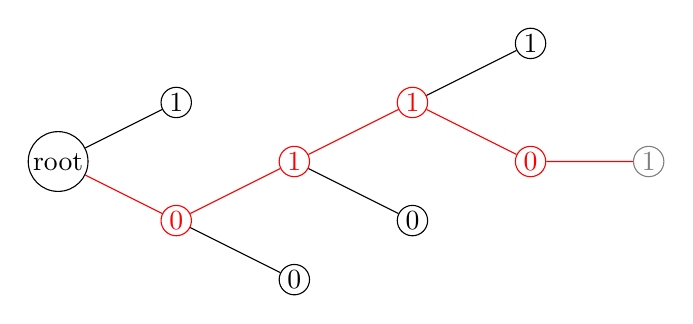
\begin{tikzpicture}
[
   every node/.style={circle,inner sep=1pt,draw}
]
\node {root} [grow=right]
  child [red] {node {0}
    child [black] {node {0}}
    child [red] {node {1}
      child [black] {node {0}}
      child [red] {node {1}
	child [red] {node {0}
	  child [red] {node [circle,gray,draw] {1}}
	}
	child [black] {node {1}}
      }
    }
  }
  child {node {1}};
\end{tikzpicture}
\caption{Representation of a word ``01101'' in knowledgebase}
\label{knowledgebasepic}
\end{figure}


\paragraph{}	
Consider the word \texttt{01101} as marked in the tree above. When this word is added to the knowledgebase, it is not stored as a single \stringtype at a node but the symbols of the word are stored at consequtive nodes. Sequence of these symbols at depth six (starting from the root) constructs the word. Hence it is termed that the node circled gray \emph{represents} the word \texttt{01101}. In the tree, the symbol \texttt{0} is a child of the root, symbol \texttt{1} is the child of \texttt{0} and so on. The node representing the word can be reached by traversing from the root to the last child and accumulating the symbols that every node contains. Alternatively, the word can also be retrieved by ascending from a node to the root and reversing the word obtained. \libalf uses the latter technique. 
\vskip 1pt
	
\subsection{Description of the Structure}
	
The knowledgebase is as a template class enabling the use of arbitrary values for storing membership information.
The class \knowledgebase contains a class \node consisting variables necessary for the node. \node also holds internal methods which are important for both using and expanding \libalf.
\paragraph{}
The constructor of the class \node creates the root node with the following values to its attributes.
\begin{itemize}
\item \texttt{parent} \vskip 1pt A pointer variable of type \node that points to the parent of the node.
\item \texttt{label} \vskip 1pt An \integer variable that stores the symbol represented by the node.
\item \texttt{status} \vskip 1pt The variable \textbf{status} indicates whether the classification of the word represented by the node is \emph{required}, \emph{answered} or can be \emph{ignored}. \\ Since the knowledgebase is a prefix tree, it stores not only the supplied words but also the prefixes of the word. However, the classification of these prefixes may not be of interest and can be \emph{ignored}. On the otherhand, learning algorithm creates queries that are to be resolved. Status of such words are set as \emph{required}. Hence, the variable differentiates these words. For this purpose, it is an \texttt{enum} type variable that can take one of three values ``NODE\_IGNORE'', ``NODE\_REQUIRED'' and ``NODE\_ANSWERED''. 
\item \texttt{ans} \vskip 1pt The variable stores the answer (or the acceptance criteria / classification) of the node. 
\end{itemize}	


\subsection{Methods in Detail}
This section describes methods that are more useful for extending \libalf. These methods mostly emphasize on operations that can be performed over the node, methods on handling words, classifications and queries. A complete list of methods and their explanation is provided in the next section.

\subsection*{Creating the Root node}
The root node is initialized when the knowledgebase is created. The constructor of class \node defines the following properties for its attributes.
\begin{itemize}
\item \textbf{node::node(knowledgebase * base)} \vskip 1pt
The method sets the following properties to the root node.
\begin{enumerate}
\item parent = NULL ; root node does not have a parent.
\item label = -1 ; which is equivalent to epsilon
\item status = STATUS\_IGNORE ; the acceptance rule or classification of the root node is initially not necessary.
\end{enumerate}	
\end{itemize}

\subsection*{Working with Nodes}
The child nodes are structured as \vectored type \node variable called \texttt{children}. Methods operating on the nodes are mostly internal methods and cannot be accessed publicly.
\begin{enumerate}
\item \textbf{node::node* get\_next(node * current\_child)} \vskip 1pt
The method returns the next node or the next child of the current node (which is passed as an arguement). 
	
\item \textbf{node::node * get\_parent()} \vskip 1pt
The method returns the parent of the current node.

\item \textbf{node::list$<$int$>$ get\_word()} \vskip 1pt
The method returns the word that the current node represents. The method traverses backwards in the tree (ascending from child to parent) and reverses the sequence obtained to build the correct word.
	
\item \textbf{node::int get\_label()} \vskip 1pt
The method returns the label of the node.
	
\item \textbf{node::node * find\_child(int label)} \hfill \vskip 1pt
The method finds the child node with the specified label.
	
\item \textbf{node::node * find\_descendant(list$<$int$>$ :: iterator infix\_start, list<int>::iterator infix\_limit)} \hfill \vskip 1pt
The method finds the child node specified by a word and returns it. It traverses through the tree based on the iteration over the word to find the path that generates the required word.
	
\item \textbf{knowledgebase::node* get\_rootptr()} \hfill \vskip 1pt
The method returns the pointer to the root node of the knowledgebase.
	
\item \textbf{knowledgebase::node* get\_nodeptr(list$<$int$>$ \& word)} \hfill \vskip 1pt
The method returns the pointer to the current node specified by the word as the parameter.
	
\end{enumerate}

\subsection*{Words and Classification}

The primary purpose of the knowledgebase is centered on storing words and classifications which constitutes the first source for a learning algorithm to compute a conjecture. Methods related to this function are listed below.
	
\begin{enumerate}
\item \textbf{node::node * find\_or\_create\_child(int label)} \vskip 1pt
	This function returns the child node given the label. If the node does not exist, it creates the child node with the specified label.
	
\item \textbf{node::node * find\_or\_create\_descendant(list$<$int$>$::iterator infix\_start, list$<$int$>$::iterator infix\_limit)} \hfill \vskip 1pt
	This function behaves almost similar to the previous one. The difference is that it does not operate on a single label but on a word (which is a list of \integer). 
\end{enumerate}	

 The method \texttt{add\_knowledge} simply calls the method \texttt{find\_or\_create\_descendant} so that the knowledge will be added only information about the word does not already exist in the knowledgebase.


\subsection*{Handling Queries}
In addition to the already discussed query handling methods, the ones discussed below is of most interest for expanding \libalf. 
As already mentioned, query handling mainly depends on the \texttt{status} of the word. The following methods operate on this aspect. 
\begin{enumerate}
\item \textbf{node::bool mark\_required()} \vskip 1pt
The method returns \true if the acceptance or the classification of the node is \emph{requried} (i.e, ``status'' is NODE\_REQUIRED). It returns \false if the classification is already known.
	
\item \textbf{node::bool is\_required()} \vskip 1pt
The method returns the ``status'' as \texttt{NODE\_REQUIRED}. It is used to set this status to a particular node under consideration.

\item \textbf{node::bool is\_answered()} \vskip 1pt
The method returns the ``status'' as \texttt{NODE\_ANSWERED}. It is used to set this status to a particular node under consideration.
	
\item \textbf{node::answer get\_answer()} \vskip 1pt
The method returns the \emph{answer} (classification of the node) stored for the node. 
\end{enumerate}

\vskip 1pt
The following methods describe the operations associated with queries.

\begin{enumerate}

\item \textbf{knowledgebase::int add\_query(list$<$int$>$ \& word, int prefix\_count = 0)} \vskip 1pt
The method is primarily used to add a query to the knowledgebase. When a query is generated, the method first checks if that word already exists with its classification in the knowledgebase (by using the \texttt{find\_or\_create\_child(int label)} method). Hence, if the classification of the word is unknown and does not already exist, the corresponding node will be created and eventually added in the query tree (since this method is used by \texttt{create\_query\_tree(\ldots)}.
  	
\item \textbf{knowledgebase::bool resolve\_query(list$<$int$>$ \& word, answer \& acceptance) and bool resolve\_or\_add\_query(list$<$int$>$ \& word, answer \& acceptance)} \hfill \vskip 1pt
These two methods can be described together as their functionality is almost similar and differ only in one aspect. Both methods return \true if the classification of the word is already known and \false if it is unknown. While ``resolve\_query()'' only returns \false, ``resolve\_or\_add\_query()'' marks the status of this word as required and then returns \false. Naturally, the former uses ``find\_descendant()'' and the latter makes use of ``find\_or\_create\_descendant()''.

\item \textbf{knowledgebase::void clear\_queries()} \hfill \vskip 1pt
This method is used to remove all the nodes that are identified or marked as a query.
\end{enumerate}
\vskip 1pt
\vskip 1pt

\subsection*{Alphabet in Knowledgebase}
The section gives an extended view of the concept of alphabet size in the knowledgebase. In principal, the knowledgebase does not store the alphabet size of the conjecture specified by the user. The knowledgebase does not work only based on the alphabet size specified by the user and is capable of constructing the tree even if symbols outside the alphabet set are input. The knowledgebase can identify the rise in the alphabet size and record the largest symbol in the tree. But, such improper input will lead the learning algorithm to compute incorrect conjecture.

\begin{enumerate}
\item \textbf{knowledgebase::int get\_largest\_symbol()} \vskip 1pt
The method has already been described in the section on user's perspective. Deepening into the concept behind it, the method simply returns what is available in the variable ``largest\_symbol''. It does not check whether the alphabet size has been modified. A good way to do that would be to use the methods listed below.
	
\item \textbf{knowledgebase::int check\_largest\_symbol()} \hfill \vskip 1pt
The method performs a check on the knowledgebase and realizes the largest symbol that is currently available. Hence, if there was a change in the size of the alphabet at some point of time, it is automatacially adjusted when this method is called.
	
\item \textbf{bool cleanup()} \hfill \vskip 1pt
The method cleans the knowledgebase by removing all the unnecessary branches i.e, branches that consists only of IGNORE as the status. This is an example for a method that can cause a change in the largest symbol. If the branches containing a particular symbol are removed in the clean up, it subsequentely causes a change in the largest symbol. 
\end{enumerate}

\subsection*{Displaying the knowledgebase}
Having described two methods in the previous section on the same topic, what is listed below is another method that is mostly of interest to a developer. 
\begin{itemize}
 \item \textbf{void print(ostream \&os)} \vskip 1pt
  This method prints the knowledgbase to any kind of an output stream. It prints the word, its status and the answer of all the words available in the knowledgebase.
\end{itemize}

\vskip 1pt
The methods described above summerizes the most important methods from the view of a developer.
	
\section{Methods Specifications}
The section supplies a comprehensive list of all the methods used in the knowledgebase along account of their particulars. The section is divided based on on the class that the methods belong to.
\subsection{Class - \node}
\begin{enumerate}
%%%
\item \begin{detail}
{get\_next}
{node* get\_next(node * current\_child)}
{current\_child - The current child}
{Returns the next node} 
\end{detail}
%%%
\item \begin{detail}
{Constructor}
{node(knowledgebase * base)}
{base - the name of the knowledgebase}
{Creates the root node of the knowledgebase and sets its \texttt{parent} to NULL} 
\end{detail}
%%%
\item \begin{detail}
{get\_parent}
{node * get\_parent()}
{--}
{Returns the parent of the node that calls this function} 
\end{detail}
%%%
\item \begin{detail}
{find\_child}
{node * find\_child(int label)}
{label - the label that the child node must contain}
{Returns the node that contains the label specified as the parameter} 
\end{detail}
%%%
\item \begin{detail}
{find\_descendant}
{node * find\_descendant(list$<$int$>$::iterator infix\_start,\\ list$<$int$>$::iterator infix\_limit)}
{infix\_start - the word or symbol that is the starting point \\ infix\_limit - the word which is to be found}
{Returns the node that represents the word infix\_limit} 
\end{detail}
%%%
\item \begin{detail}
{find\_or\_create\_child}
{node * find\_or\_create\_child(int label)}
{label - the label that the child node must contain}
{Returns the node that contains the label specified as parameter. If not found, it creates such a node and returns it.} 
\end{detail}
%%%
\item \begin{detail}
{serialize\_subtree}
{void serialize\_subtree(basic\_string$<$int32\_t$>$ \& into)}
{\texttt{into} - the string that contains the serialized trees of the knowledgebase}
{Converts the subtree into \stringtype and appended to \texttt{into}. This method is used during serialization} 
\end{detail}
%%%
\item \begin{detail}
{deserialize\_subtree**}
{bool deserialize\_subtree(basic\_string$<$int32\_t$>$::iterator \& it, \\ basic\_string$<$int32\_t$>$::iterator limit, int \& count)}
{
\texttt{it} - iterator to iterate over the string containing the word \\
\texttt{limit} - the last word that the subtree contains
\texttt{count} - \integer to count the subtrees
 }
{Returns \true after deserializing the subtrees. Returns \false if \texttt{it} and \texttt{limit} are equal.} 
\end{detail}
%%%
\item \begin{detail}
{get\_selfptr}
{node * get\_selfptr()}
{--}
{A self pointer that returns its own node.} 
\end{detail}
%%%
\item \begin{detail}
{max\_child\_count}
{int max\_child\_count()}
{--}
{Returns the maximum number of children existing in the knolwedgebase. If it returns ``n'', it implies that there may exist [0..n] suffixes.} 
\end{detail}
%%%
\item \begin{detail}
{has\_specific\_suffix}
{bool has\_specific\_suffix(answer specific\_answer)}
{\texttt{specific\_answer} - the answer that needs to be compared}
{Checks if a specific suffix/word has a specific answer. Returns \true if such a case exists, otherwise returns \false.} 
\end{detail}
%%%
\item \begin{detail}
{get\_label}
{int get\_label()}
{--}
{Returns the label of this node (which is the last symbol of the word that this node represents).} 
\end{detail}
%%%
\item \begin{detail}
{get\_word}
{list<int> get\_word()}
{--}
{Returns the word that this node represents.} 
\end{detail}
%%%
\item \begin{detail}
{mark\_required}
{bool mark\_required()}
{--}
{Returns \true if answer to this node is required. Returns \false if the answer is already known.} 
\end{detail}
%%%
\item \begin{detail}
{is\_required}
{bool is\_required()}
{--}
{Returns \true if this node is marked unknown and required, \false otherwise.} 
\end{detail}
%%%
\item \begin{detail}
{is\_answered}
{bool is\_answered()}
{--}
{Returns \true if this node is already answered, \false otherwise.} 
\end{detail}
%%%
\item \begin{detail}
{set\_answer}
{bool set\_answer(answer ans)}
{\texttt{ans} - answer that must be set.}
{Returns \true if the node is already answered and the answer is same as \texttt{ans}, otherwise \false. If the node is not answered already, then it returns \true after setting \texttt{ans} as the answer.} 
\end{detail}
%%%
\item \begin{detail}
{get\_answer}
{answer get\_answer()}
{--}
{Returns the answer of this node.} 
\end{detail}
%%%
\item \begin{detail}
{no\_subqueries}
{bool no\_subqueries(bool check\_self = true)}
{\texttt{check\_self} - Set to true. Used to check if the status of this node is marked required. }
{Returns \true if there are any queries with this node as the prefix, \false otherwise. Also returns \false if this node is not answered and marked required.} 
\end{detail}
%%%
\item \begin{detail}
{different}
{bool different(node * other)}
{\texttt{other} - a node whose answer needs to be compared to the current node. }
{Returns \true if this node and \texttt{other} node have the same answer, \false otherwise. } 
\end{detail}
%%%
\item \begin{detail}
{recursive\_different}
{bool recursive\_different(node * other, int depth)}
{\texttt{other} - a node whose answer needs to be compared to the current node.
 \texttt{depth} - the depth of the tree that indiciates the length of the word. }
{Compares the answers of the two nodes and their children upto a level specified by \texttt{depth}. Returns \true if there are no inconsistancies in the answers, \false otherwise. } 
\end{detail}
%%%
\item \begin{detail}
{is\_prefix\_of}
{bool is\_prefix\_of(node*other)}
{\texttt{other} - a node whose answer needs to be compared to the current node.}
{Retruns \true if this node is a suffix of the \texttt{other} node. } 
\end{detail}
%%%
\item \begin{detail}
{is\_suffix\_of}
{bool is\_suffix\_of(node*other)}
{\texttt{other} - a node whose answer needs to be compared to the current node.}
{Retruns \true if this node is a preffix of the \texttt{other} node. } 
\end{detail}
%%%
\item \begin{detail}
{get\_memory\_usage}
{unsigned long long int get\_memory\_usage()}
{--}
{Retruns the size of the memory used by this subtree. } 
\end{detail}
%%%
\item \begin{detail}
{ignore}
{void ignore()}
{--}
{Changes the status of this node to NODE\_IGNORE. } 
\end{detail}
%%%
\item \begin{detail}
{cleanup}
{bool cleanup()}
{--}
{Returns \true after deleting all the branches that has status as NODE\_IGNORE. } 
\end{detail}
%%%
\end{enumerate}

\subsection{Class - \texttt{iterator}}
\begin{enumerate}
\item \begin{detail}
{iterator}
{iterator()}
{--}
{Sets this node to NULL and initializes an iterator to the last node that is marked required. } 
\end{detail}
%%%
\item \begin{detail}
{iterator}
{iterator(const iterator \& other)}
{--}
{Sets the values of this node to those of the \texttt{other} node.} 
\end{detail}
%%%
\item \begin{detail}
{iterator**}
{iterator(bool queries\_only, typename list$<$node*$>$::iterator currentquery, node * current, knowledgebase * base)}
{\texttt{queries\_only} - a boolean variable that is \true if queries exist and \false if there are no queries in the knowledebase
 \texttt{currentquery} - iterator to iterate over queries
 \texttt{current} - the node under consideration
 \texttt{base} - the knowledgebase that is being processed.}
{Sets the values of this node to those specified in the arguement.} 
\end{detail}
%%%
\item \begin{detail}
{operator++}
{iterator \& operator++()}
{--}
{Operator overloading applied to ``++''. Creates an iterator that points to the next query and returns the node} 
\end{detail}
%%%
\item \begin{detail}
{operator++ **}
{iterator operator++(int foo)}
{--}
{--} 
\end{detail}
%%%
\item \begin{detail}
{is\_valid()}
{bool is\_valid()}
{--}
{Returns \true if the current iterator is not NULL, \false otherwise.} 
\end{detail}
%%%
\item \begin{detail}
{operator*}
{node \& operator*()}
{--}
{Returns the pointer to the current iterator.} 
\end{detail}
%%%
\item \begin{detail}
{operator-$>$}
{node * operator-$>$()}
{--}
{Returns the current iterator.} 
\end{detail}
%%%
\item \begin{detail}
{operator=}
{iterator \& operator=(const iterator \& it)}
{\texttt{it} - an iterator}
{Creates an iterator with the values of iterator \texttt{it} and returns this. } 
\end{detail}
%%%
\item \begin{detail}
{operator==}
{bool operator==(const iterator \& it)}
{\texttt{it} - an iterator}
{Returns \true if the current iterator is same as \texttt{it}, \false otherwise.} 
\end{detail}
%%%
\item \begin{detail}
{operator!=}
{bool operator!=(const iterator \& it)}
{\texttt{it} - an iterator}
{Returns \true if the current iterator is not equal to \texttt{it}, \false otherwise.} 
\end{detail}
\end{enumerate}



\subsection{Class - \knowledgebase}
\begin{enumerate}
%%%
\item \begin{detail}
{knowledgebase}
{knowledgebase()}
{--}
{Creates a knowledgebase with root as NULL.} 
\end{detail}
%%%
\item \begin{detail}
{knowledgebase}
{\~knowledgebase()}
{--}
{Deletes the knowledgebase by deleting the root.} 
\end{detail}
%%%
\item \begin{detail}
{clear}
{void clear()}
{--}
{Deletes the existing knowledgebase and creates a new knowledgebase containing only the root.} 
\end{detail}
%%%
\item \begin{detail}
{clear\_queries}
{void clear\_queries()}
{--}
{Deletes all the nodes that are marked as queries.} 
\end{detail}
%%%
\item \begin{detail}
{undo**}
{bool undo(unsigned int count)}
{\texttt{count} - }
{Used to undo the last operation.} 
\end{detail}
%%%
\item \begin{detail}
{get\_memory\_usage}
{unsigned long long int get\_memory\_usage()}
{--}
{Returns the memory used by the knowledgebase.} 
\end{detail}
%%%
\item \begin{detail}
{is\_answered}
{bool is\_answered()}
{--}
{Returns \true if there are no nodes marked required, \false otherwise.} 
\end{detail}
%%%
\item \begin{detail}
{is\_empty}
{bool is\_empty()}
{--}
{Returns \true if there are no nodes marked required and answered (the tree is empty), \false otherwise.} 
\end{detail}
%%%
\item \begin{detail}
{count\_nodes}
{int count\_nodes()}
{--}
{Returns the number of nodes present in the knowledgebase.} 
\end{detail}
%%%
\item \begin{detail}
{count\_answers}
{int count\_answers()}
{--}
{Returns the number of nodes that are already answered in the knowledgebase.} 
\end{detail}
%%%
\item \begin{detail}
{count\_queries}
{int count\_queries()}
{--}
{Returns the number of nodes that are marked required in the knowledgebase.} 
\end{detail}
%%%
\item \begin{detail}
{count\_resolved\_queries}
{int count\_resolved\_queries()}
{--}
{Returns the number of answered nodes that were once marked required.} 
\end{detail}
%%%
\item \begin{detail}
{reset\_resolved\_queries}
{void reset\_resolved\_queries()}
{--}
{Resets the number of resolved queries to zero.} 
\end{detail}
%%%
\item \begin{detail}
{get\_largest\_symbol}
{int get\_largest\_symbol()}
{--}
{Returns the largest symbol that is present in the knowledgebase. Essentially, this returns the number which is one less than the alphabet size.} 
\end{detail}
%%%
\item \begin{detail}
{check\_largest\_symbol}
{int check\_largest\_symbol()}
{--}
{Adjusts the largest symbol present in the knowledgebase and returns it.} 
\end{detail}
%%%
\item \begin{detail}
{print}
{void print(ostream \&os)}
{\texttt{os} - an output stream.}
{Prints the knowledgebase on the screen. Prints the word, status and the answer of all the words stored in the knowledgebase.} 
\end{detail}
%%%
\item \begin{detail}
{tostring}
{string tostring()}
{--}
{Used to return a string stream for serialization.} 
\end{detail}
%%%
\item \begin{detail}
{generate\_dotfile}
{string generate\_dotfile()}
{--}
{Generates the ``.dot'' file of the knowledgebase for graphical representation.} 
\end{detail}
%%%
\item \begin{detail}
{serialize}
{basic\_string$<$int32\_t$>$ serialize()}
{--}
{Returns a string which represents the complete knowledgebase.} 
\end{detail}
%%%
\item \begin{detail}
{deserialize**}
{bool deserialize(basic\_string$<$int32\_t$>$::iterator \&it, \\ basic\_string$<$int32\_t$>$::iterator limit)}
{\texttt{it} - iterator to iterate over the string containing the word.
 \texttt{limit} - iterator that points to the last word }
{Returns \true if the string was deserialized to knowledgebase successfully, \false if the deserialization failed.} 
\end{detail}
%%%
\item \begin{detail}
{deserialize\_query\_acceptances}
{bool deserialize\_query\_acceptances(basic\_string$<$int32\_t$>$::iterator \&it,\\ basic\_string$<$int32\_t$>$::iterator limit)}
{\texttt{it} - iterator to iterate over the string containing the word.
 \texttt{limit} - iterator that points to the last word }
{Returns \true after answering all the queries in the knowledgebase from a single serialized data. } 
\end{detail}
%%%
\item \begin{detail}
{create\_query\_tree}
{knowledgebase * create\_query\_tree()}
{--}
{Returns a tree created by adding to this tree, all the words marked as required in the knowledgebase.} 
\end{detail}
%%%
\item \begin{detail}
{get\_queries}
{list$<$list$<$int$>$ $>$ get\_queries()}
{--}
{Returns a list of list of \integer that consists of all the queries existing in the knowledgebase.} 
\end{detail}
%%%
\item \begin{detail}
{merge\_knowledgebase}
{bool merge\_knowledgebase(knowledgebase \& other\_tree)}
{\texttt{other\_tree} - the tree to be merged.}
{Returns \true if the current tree could be merged with the \texttt{other\_tree}, \false otherwise. Two trees can be merged only if they are consistant. This method merges only answered information, it does not merge the queries. } 
\end{detail}
%%%
\item \begin{detail}
{add\_knowledge}
{bool add\_knowledge(list$<$int$>$ \& word, answer acceptance)}
{\texttt{word} - the word to be added to the knowledgebase.
 \texttt{acceptance} - the classification of the word.}
{Returns \true if the knowledge for this word does not already exist and is successfully added to the knowledgebase, \false otherwise.} 
\end{detail}
%%%
\item \begin{detail}
{add\_query}
{int add\_query(list$<$int$>$ \& word, int prefix\_count = 0)}
{\texttt{word} - the word/query to be added to the knowledgebase.
 \texttt{prefix\_count} - initialized to zero. It is the count of all the prefixes that can be formed with the word.}
{Creates the query and the necessary prefixes (which will also be marked as a query) and returns the total number of queries formed.} 
\end{detail}
%%%
\item \begin{detail}
{resolve\_query}
{bool resolve\_query(list$<$int$>$ \& word, answer \& acceptance)}
{\texttt{word} - the word/query to be added to the knowledgebase.
 \texttt{acceptance} - the classification of the word.}
{If the word is already known and is answered, then the answer is assigned to \texttt{acceptance} and returns \true, otherwise returns \false.} 
\end{detail}
%%%
\item \begin{detail}
{resolve\_or\_add\_query}
{bool resolve\_or\_add\_query(list$<$int$>$ \& word, answer \& acceptance)}
{\texttt{word} - the word/query to be added to the knowledgebase.
 \texttt{acceptance} - the classification of the word.}
{Returns \true if the word is already known and answered, else marks the word as required and returns \false.} 
\end{detail}
%%%
\item \begin{detail}
{get\_nodeptr}
{node* get\_nodeptr(list$<$int$>$ \& word)}
{\texttt{word} - a word.}
{Returns the node that represents this word.} 
\end{detail}
%%%
\item \begin{detail}
{get\_rootptr}
{node* get\_rootptr()}
{--}
{Returns the root.} 
\end{detail}
%%%
\item \begin{detail}
{begin}
{iterator begin()}
{--}
{Returns an iterator that begins at the root node.} 
\end{detail}
%%%
\item \begin{detail}
{end}
{iterator end()}
{--}
{Returns an iterator which is used to point to the last node.} 
\end{detail}
%%%
\item \begin{detail}
{qbegin}
{iterator qbegin()}
{--}
{Returns an iterator that begins at the first node that is marked required.} 
\end{detail}
%%%
\item \begin{detail}
{qend}
{iterator qend()}
{--}
{Returns an iterator which is used to point to the last node that is marked required.} 
\end{detail}
\end{enumerate}

%%%%%%%%--------------------------------------------------------%%%%%%%%%%

%\textbf{methods not described} \vskip 1pt
%bool is\_lex\_smaller(node * other) \\
%bool is\_graded\_lex\_smaller(node * other) \\
%unsigned int get\_timestamp() \\
%string generate\_dotfile(equivalence\_relation \& eq) \\
%equivalence relation class\\
%class kIterator\_lex\_graded 

%%%%%%%%--------------------------------------------------------%%%%%%%%%%

\chapter{Learning Algorithms}

A learning algorithm is a component that retrieves the desired information from the knowledgebase to construct a conjecture. 
The common objective of all learning algorithms is to generalize knowledge gained throughout a learning process. In such a process, the learning algorithm is confronted with classified examples. They are utilized to derive a hypothesis which is able to classify new examples in conformance with the examples already seen.
\paragraph{}
A knowledgebase and a learning algorithm are associated in such a way that queries can be exchanged between them. Unlike other learning libraries, libalf is not restricted to a strict one-to-one relationship between a knowledgebase and a learning algorithm, but
also features one-to-many relationships. This allows us to experiment with different learning techniques on the same data set with only a minimum of effort. This facilitates the learning algorithms to be used in a plug and play fashion.

\section{The Types of Algorithms - An Overview}

A conventional way to distinguish learning algorithms is to group them into \online and \offline algorithms. Online learning techniques are capable of actively asking queries to some kind of teacher who is able to classify these queries. Offline algorithms, on the other hand, are passively provided with a set of classified examples from which they have to build the conjecture.

\subsection{Online Algorithms}

Online learning algorithms build the conjecture by actively asking queries to a \teacher (or a user). Queries are of two types - membership queries and equivalence queries. The teacher is required to \emph{resolve} the memebership query by providing the classification of the given word.
Equivalence queries check whether a derived conjecture is an equivalent description of the target language to be inferred.
The working of such an algorithm can be described in the following steps. An algorithmic workflow is provided later in this chapter.
\begin{itemize}
 \item The algorithm runs on iteration which begins at making an \emph{advance} where in the algorithm tries to compute a conjecture with information available in the knowledgebase.
 \item This leads to the rise of membership queries if no conjecture was created. These queries are resolved by the teacher, answer added to the knowledgebase and the algorithm continues the iteration.
 \item On the other hand, if a conjecture was computed, it is presented to the teacher. The algorithm terminates if the conjecture is correct. Otherwise, the iteration continues after the teacher renders a counter example.
\end{itemize}

\subsection{Offline Algorithms}

Offline algorithms, in contrast to the online variant, is an NP complete problem of finding the smallest DFA consistant with a given set of classified words.
The algorithm is provided with a set S of classified words (called samples) and the algorithm derives a conjecture which conforms to these samples. More precisely, this means that all positive examples from S are recognized (or accepted) and all negative examples are rejected by the conjecture. 
\paragraph{}
The working of this algorithm follows a simple two step procedure. 
\begin{itemize}
 \item The knowledgebase is furnished with all samples. 
 \item The algorithm is then made to advance to compute the conjecture conforming to the samples. 
\end{itemize}

\subsection{List of Algorithms}

As of \today, \libalf implements seven algorithms for both deterministic and non deterministic automata as listed in the table \ref{algtables1}

\begin{table} [h]
\centering
\begin{tabular}[c]{lcr}
\toprule[1pt]
Online Algorithms & Offline Algorithms \\	
\midrule
Angluin's L [2] (two variants) & Biermann [3] \\
NL [4] & RPNI [13] \\
Kearns / Vazirani [10] & DeLeTe2 [6]\\
\bottomrule[1pt]
\end{tabular}
\caption{List of Algorithms Implemented}
\label{algtables1}
\end{table}

---------------------------------------------------------------------------------------------------

\subsection{Methods}

Constructor used to initialize the learning algorithm. \vskip 1pt

\paragraph{learning\_algorithm()}
It initializes the essentials for a learning algorithm such as, pointer to the knowledgebase, normalizer and logger. 
do\_timing - to create timing statistics this has to be set true
in\_timing - variable to check if the currently timing statistics are being measured.
alphabet\_size - the alphabet size of the conjecture to be computed.


The constructor of all the learning algorithms usually perform three tasks. They set the pointer to the knowledgebase, set the logger and the alphabet size. 

\paragraph{virtual void set\_alphabet\_size(int alphabet\_size)}
method that sets the alphabet size for computing the conjecture. This method is used only during the initial setting of the learning algorithm. 

\paragraph{virtual void increase\_alphabet\_size(int new\_asize)}
The method increases the size of the alphabet to a new value.

\paragraph{virtual int get\_alphabet\_size()}
Returns the alphabet size of the conjecture.

\paragraph{virtual void set\_logger(logger * l)}
If the value of ``l'' is not NULL, then it is set as the logger. Otherwise, the logger is set to ``ignore'' which implies that no logger exists.

\paragraph{virtual void set\_knowledge\_source(knowledgebase $<$answer$>$ * base)}
Sets the source (the knowledgebase) which consists of all the membership information to the learning algorithm.

\paragraph{virtual knowledgebase$<$answer$>$ * get\_knowledge\_source()}
Returns the pointer to the knowledgebase which is currently the source of membership information.

\paragraph{virtual void set\_normalizer(normalizer * norm)}
Sets the normalizer to the one pointed by the arguement ``norm''.

\paragraph{virtual void unset\_normalizer()}
Sets the normailizer to NULL. 

\paragraph{virtual memory\_statistics get\_memory\_statistics()}
Returns the memory statistics.

\paragraph{virtual timing\_statistics get\_timing\_statistics()}
Returns the timing statistics which is stored in the variable ``current\_stats''.

\paragraph{virtual void enable\_timing()}
Enables the maintenance of timing statistics by setting the ``do\_timing'' variable to be \true.

\paragraph{virtual void disable\_timing()}
Disables the maintenance of timing statistics by setting the ``do\_timing'' variable to be \false.

\paragraph{virtual void reset\_timing()}
The ``current\_stats'' is reset.

\paragraph{virtual bool sync\_to\_knowledgebase()}
Knowledgebase may support undo operation. In such a case the learning algorithm needs to stay synchronized with the knowledgebase failing to which it may return erroneaous output. The method checks the knowledgebase if there is any knowledge and then checks its internal knowledge, removes the obsolete knowledge, changes its state (delete rows/columns etc.) to be synchronized with the knowledgebase and returns \true. If it returns \false, the algorithm is in undefined state and must not be used anymore. This method should be called after each undo opearation performed in the knowledgebase.

\paragraph{virtual bool supports\_sync()}
 Checks whether the learning algorithm supports synchronization with the associated Knowledgebase. Returns \true if undo operations on the knowledgebase are allowed. Each undo-operation has to be followed by a call to sync\_to\_knowledgebase(). Otherwise returns \false.

\vskip 1pt
Building the conjecture \vskip 1pt

\paragraph{virtual bool complete()}
The method is used by the learning algorithm to complete the table in such a way that a conjecture can be derived from it. Returns true if the table is complete. Returns \false if the table is incomplete due to missing knowledge. 

\paragraph{virtual conjecture * derive\_conjecture()}
The methodd derives a conjecture from the given data structure available in the knowledgebase. 

\paragraph{virtual bool conjecture\_ready()}
Returns \true if a conjecture can be constructed without any further queries. Otherwise, returns \false.

\paragraph{virtual conjecture * advance()}
The most important method of . The method first tries to complete the table. If all knowledge was available, then it tries to derive a conjecture and when a conjecture is ready, it is returned. If the table was unable to be completed, then unknown knowledge is marked required and NULL is returned.

\paragraph{virtual bool add\_counterexample(list$<$int$>$)}
The method is used by \online algorithms when a computed conjecture is declined by the teacher, i.e. when the equivalence query is answered negative. The counter example provided by the user is first processed by the learning algorithm which marks it as a membership query and is added to the knowledgebase. \\
This method is used only by an \online algorithm. For \offline algorithms, this method is a stub.

\paragraph{virtual basic\_string$<$int32\_t$>$ serialize()}
The method returns a \stringtype composed of \integer containing the serialization of the state of the learning algorithm.

\paragraph{virtual bool deserialize(basic\_string$<$int32\_t$>$::iterator \& it, basic\_string$<$int32\_t$>$::iterator limit)}
Restores the data of a serialized learning algorithm. The current state of the learning algorithms is discarded. \\
The method returns \true if the deserialization was successfull. Otherwise, returns \false.

\chapter{Loggers \& Statistics}

A \textbf{Logger} is an adjustable logging facility that an algorithm can write to. This eases the application debugging and development. When a learning algorithm is initialized, a logger is associated with it along with the knowledgebase. \libalf provides flexible logger implementations for the user. A learning algorithm can either use an output stream or a buffer as the logger. One may also choose to ignore the logger. \\
\textbf{Statistics} refers to the statistical data that can be acquired by evaluating the learning procedure. Information about the memory usage, queries produced, time taken for computing conjecture and other details may serve as base for analysing the learning algorithm in various cases. 

\section{Logger Implementation}
A loglevel marks the state of a particular log message. An \emph{enum} type variable logger\_loglevel is used to define the messages with the following attributes.
\begin{itemize}
 \item \textbf{LOGGER\_INTERNAL=0} ; (An internal method)
 \item \textbf{LOGGER\_ERROR = 1} ; All log messages that describe a non-recoverable error are marked with this.
 \item \textbf{LOGGER\_WARN = 2} ; Messages describing a state or command that is erroneous but may be ignored under most conditions.
 \item \textbf{LOGGER\_INFO = 3} ; Any information that does not describe an erroneous condition.
 \item \textbf{LOGGER\_DEBUG = 4} ; Messages that may help debugging of libalf.( Most likely removed before release version ).
 \item \textbf{LOGGER\_ALGORITHM = 5} ; (Do not use this as minimal loglevel)
\end{itemize}

\subsection{class Logger}
The main class that consists of attributes and methods to implement the logger. 

\subsection*{Attributes} 
It consists of two attributes that every type of logger makes use of.
\begin{enumerate}
 \item \textbf{enum logger\_loglevel minimal\_loglevel} - a minimal setting of the loglevel
 \item \textbf{bool log\_algorithm} - An boolean variable to indicate if a logger is to be associated with an algorithm or not.
\end{enumerate}

\subsection*{Methods}
The following methods are defined in the class.
\begin{enumerate}
 \item \textbf{void set\_minimal\_loglevel(enum logger\_loglevel minimal\_loglevel)} \\
	Sets the minimum logger level using the attributes loglevel attributes.
 \item \textbf{void set\_log\_algorithm(bool log\_algorithm)} \\
	The method sets logger for the algorithm based if the arguement is \true. It ignores the logger if the parameter is \false. 
 \item \textbf{virtual void operator()(enum logger\_loglevel, string\&)} and \textbf{virtual void operator()(enum logger\_loglevel, 	const char* format, ...)} \\
	The method takes the logger type and message as parameters for entry to the logger. If other variables also need to be used, it can be done so using the second method. 
\end{enumerate}

\subsection*{Example}
\begin{lstlisting}
if(my_knowledge == NULL) 
{
(*my_logger)(LOGGER_ERROR, "learning_algorithm::advance()  
	      no knowledgebase was set!\n");
return false; 
}
\end{lstlisting}
The above code snipped is an extraction from the ``advance()'' method of the learning algorithm. When no knowledgebase is set to the algorith, it enters the message ``learning\_algorithm::advance(): no knowledgebase was set'' to the log ``my\_logger'' and marks it as an error with ``LOGGER\_ERROR''. 
\vskip 1pt
All three types of loggers are implemented with the respective classes, \texttt{ignore\_logger}, \texttt{ostream\_logger} and \texttt{buffered\_logger}. All the classes inherit the \texttt{logger} class. \\

\subsection{class ignore\_logger}
A class that does not consist of any methods. In this case, the logger is just ignored.

\subsection{class ostream\_logger}
The class consists of method to write the message to an output stream. 
\begin{itemize}
 \item \textbf{ostream\_logger(ostream *out, enum logger\_loglevel minimal\_loglevel, bool log\_algorithm = true, bool use\_color = true)} \vskip 1pt
	The method creates an output stream for the logger. The parameter \texttt{*out} points to the output stream and the minimal loglevel indicates the initial setting. The parameter \texttt{log\_algorithm} is set to \true since the logger will be used by the algorithm. The parameter \texttt{use\_color} is set to \true so that on a console output, you may view the messages in different colors!
\end{itemize}

\subsection{class buffered\_logger}
The class consists of methods for setting a buffer as a log. It should be noted that the messages passed to the buffer will not be available until it is received and flushed explicitly.

\begin{enumerate}
 \item \textbf{buffered\_logger(enum logger\_loglevel minimal\_loglevel, bool log\_algorithm = true)} \\
	The method sets the buffered logger with the minimal loglevel. \texttt{log\_algorithm} is set to \true.
 \item \textbf{string * receive\_and\_flush()} \\
	The method receives and flushes the buffered stream.
\end{enumerate}

\section{Statistics}
The library consists of four classes - \texttt{statistics}, \texttt{timing\_statistics}, \texttt{memory\_statistics} and \texttt{query\_statistics}, each of them defined in the following way. Every class consists of the serialization and deserialization methods. All the methods and attributes of the classes are specified \texttt{public}.

\subsection{class statistics}
The main class that contains objects of the other three classes to access the methods. 
\subsection*{Attributes}
\begin{enumerate}
 \item \textbf{query\_statistics queries} - Object to retrieve query statistics.
 \item \textbf{memory\_statistics memory} - Object to retrieve memory statistics.
 \item \textbf{timing\_statistics time} - Object to retrieve the timing statistics.
\end{enumerate}
\subsection*{Methods}
Along with the serialize and deserialize, the class defines the following method.
\begin{itemize}
 \item \textbf{void reset()}
	The method resets all the statistical information.
\end{itemize}

\subsection{class timing\_statistics}
The class consists of methods to obtain timing statistics of the learning procedure.
\subsection*{Attributes}
\begin{enumerate}
 \item \textbf{int32\_t user\_sec} - Variable to store the User time.
 \item \textbf{int32\_t user\_usec}
 \item \textbf{int32\_t sys\_sec} - Variable to store the System time.
 \item \textbf{int32\_t sys\_usec}
\end{enumerate}
\subsection*{Methods}
\begin{enumerate}
 \item \textbf{timing\_statistics()} \\
	Constructor that retrieves the timing information.
 \item \textbf{void reset()}
	The method resets all the acquired timing statistics.
\end{enumerate}

\subsection{class memory\_statistics}
The class consists of methods to obtain statistical information about the memory usage during the learning procedure. 
\subsection*{Attributes}
Most of the attributes belonging to this class are used by the Angluin algorithm.
\begin{enumerate}
 \item \textbf{int32\_t bytes} - bytes of algorithms data structure
 \item \textbf{int32\_t members} - number of membership data
 \item \textbf{int32\_t words} - number of words in table
 \item \textbf{int32\_t upper\_table} - size of upper table (if appropriate)
 \item \textbf{int32\_t lower\_table} - size of lower table (if appropriate)
 \item \textbf{int32\_t columns} - columns (if appropriate)
\end{enumerate}
\subsection*{Methods}
\begin{enumerate}
 \item \textbf{memory\_statistics()} \\
	Constructor to retrieve the memory statistics.
 \item \textbf{void reset()} \\
        The method resets all the acquired memory statistics.
\end{enumerate}

\subsection{class query\_statistics}
The class consists of methods to obtain statistical information about the queries produced during the learning procedure.
\subsection*{Attributes}
\begin{enumerate}
 \item \textbf{int32\_t membership} - Stores the number of membership queries.
 \item \textbf{int32\_t uniq\_membership}
 \item \textbf{int32\_t equivalence} - Stores the number of equivalence queries.
\end{enumerate}
\subsection*{Methods}
\begin{enumerate}
 \item \textbf{query\_statistics()} \\
	Constructor that retrieves statistics about the all queries produced.
 \item \textbf{void reset()}
	The method resets all the acquired statics about queries.
\end{enumerate}


\chapter{Filters \& Normalizers}
A knowledgebase can be associated with \textbf{filters} which can exploit domain specific properties and by that actively reduce the number of queries to the teacher during the learning phase. Such filters can be composed by logical connectors (and, or, not). \\
In contrast, \textbf{Normalizers} recognize equivalent words in a domain-specific sense to reduce the amount of knowledge that has to be stored.

\section{Implementation of Filters}
The filter is composed of the main class \texttt{filter} and classes for all logical connectors. They are template classes of type \texttt{answer}. They also implement serialization and deserialization apart from the other methods.

\subsection{Class - filter}
It is the main class that evaluates the word using the filter.

\subsection*{Attributes}
An \emph{enum} type variable \texttt{type} is used to define the filter type.
\begin{itemize}
 \item \textbf{FILTER\_NONE = 0} ; No filter associated
 \item \textbf{FILTER\_AND = 1} ; Filter type \emph{and}
 \item \textbf{FILTER\_OR = 2} ; Filter type \emph{or}
 \item \textbf{FILTER\_NOT = 3} ; Filter type \emph{not}
 \item \textbf{FILTER\_ALL\_EQUAL = 4} ; Filter type for equal words
 \item \textbf{FILTER\_REVERSE = 100} ; Filter type handling reverse of a word.
 \item \textbf{FILTER\_IDENTITY = 200} ; Identity filter **
\end{itemize}

\subsection*{Methods}
\begin{enumerate}
 \item \textbf{virtual void free\_all\_subfilter()} \\
	Method to erase all the subfilters (logical connectors) associated with the knowledgebase.
 \item \textbf{virtual enum type get\_type()} \\
	The method returns the type of filter. Returns FILTER\_NONE in this class.
 \item \textbf{virtual bool evaluate(knowledgebase$<$answer$>$ \& base, list$<$int$>$ \& word, answer \& result)} \\
	The method used to evaluate the world with the associated filter in the knowledgbase. 
\end{enumerate}

\subsection{Class - filter\_subfilter\_array}
A class that inherits the filter class to form the array of subfilters.
\subsection*{Attributes}
\begin{itemize}
 \item \textbf{list$<$filter$<$answer$>$*$>$ subfilter\_array} \\
	A list of all the subfilters associated with the knowledgebase.
\end{itemize}
\subsection*{Methods}
\begin{itemize}
 \item \textbf{virtual void free\_all\_subfilter()} \\
	The method to erase all subfilters.
 \item \textbf{virtual void add(filter$<$answer$>$ *f)} \\
	Method to add a filter into the array.
 \item \textbf{virtual void remove(filter$<$answer$>$ *f)} \\
	Method to remove a filter from the array.
\end{itemize}

\subsection{class - filter\_and}
The connector class \texttt{and}. It inherits the class \texttt{filter\_subfilter\_array}. 
\subsection*{Methods}
\begin{enumerate}
 \item \textbf{virtual enum filter$<$answer$>$::type get\_type()}
	The method returns the filter type which is FILTER\_AND.
 \item \textbf{virtual bool evaluate(knowledgebase$<$answer$>$ \& base, list$<$int$>$ \& word, answer \& result)}
	The method evaluates the word using the \texttt{and} operator.
\end{enumerate}

\subsection{class - filter\_or}
The connector class \texttt{or}. It inherits the class \texttt{filter\_subfilter\_array}. 
\subsection*{Methods}
\begin{enumerate}
 \item \textbf{virtual enum filter$<$answer$>$::type get\_type()}
	The method returns the filter type which is FILTER\_OR
 \item \textbf{virtual bool evaluate(knowledgebase$<$answer$>$ \& base, list$<$int$>$ \& word, answer \& result)}
	The method evaluates the word using the \texttt{or} operator.
\end{enumerate}

\subsection{class - filter\_not}
The connector class \texttt{not}. It inherits the class \texttt{filter\_subfilter\_array}. 
\subsection*{Attributes}
\begin{itemize}
 \item filter$<$answer$>$ * subfilter \\
\end{itemize}
\subsection*{Methods}
\begin{enumerate}
 \item \textbf{virtual void free\_all\_subfilter()} \\
	The method removes all the filters from the \texttt{subfilter}
 \item \textbf{virtual enum filter$<$answer$>$::type get\_type()} \\
	The method returns the filter type which is FILTER\_NOT.
 \item \textbf{virtual bool evaluate(knowledgebase$<$answer$>$ \& base, list$<$int$>$ \& word, answer \& result)} \\
	The method evaluates the word using the \texttt{and} operator.
 \item \textbf{virtual void set\_subfilter(filter$<$answer$>$ * f)} \\
	The method sets the \texttt{subfilter} to ``f''.
 \item \textbf{virtual void remove\_subfilter()}
	The method sets the \texttt{subfilter} to NULL.

\end{enumerate}


\section{Normalizer}

It is employed for learning algorithms using message sequence charts. 
\chapter{\jalf Java Library}

The \jalf \java library, as you may have come across in various sections in the previous chapters, is the \java implementation of \libalf. However, \jalf is not a standalone library. It is implemented as calls pointing to the \cpp \libalf objects. \\
The \jalf library can be used either locally through JNI or remotely from a server using the dispatcher. The important point to be noted here is that a few features in \jalf are not identical to \libalf. The differences exist at different levels and will be described in this section along with how to use \jalf and its developer's perspective.


\section{Source Code Structure}
The \jalf implementation can be found in \texttt{/libalf/jalf} folder of the \libalf package. The \jalf package information is as follows.
\begin{itemize}
 \item \texttt{src} - The folder contains \cpp methods of JNI calls that forwards the calls to \libalf.
 \item \texttt{include} - The header files generated using \texttt{javah} command.
 \item \texttt{java/src/de/libalf} - The files in this folder are the interfaces to the native methods.
 \item \texttt{java/src/de/libalf/jni} - The java native methods for JNI.
 \item \texttt{java/src/de/libalf/dispatcher} - The java native methods for dispatcher.
\end{itemize}

\section{\jalf - User Perspective}
In this section we will introduce how to use \jalf and explain its features.

\subsection*{Data Structures}
The data structure used in \jalf is mostly similar to that of \libalf. An important difference lies in the data structure of the knowledgebase. While it is possible to store arbitrary value types for classification in \libalf, it is possible to use only boolean values (\true or \false) can be used for storing classification information in \jalf. \\
However, other differences in data structures are handled entirely by the \jalf itself and the task does not burden on the user. 
For instance in \libalf, words were represented as list of integers. Similarly \jalf uses integer arrays, or more precisely, \texttt{jintArray} to represent the words and \texttt{LinkedList} for list of words. \jalf automatically performs the conversion during the execution.

\subsection*{The \jalf Factory}
Unlike \libalf the components are not entirely free but belong to what is called a Factory class. From an abstract point of view, this factory can be imagined as a roof under which the components can be declared and used. The following code snippet shows an example of how to use the factory class. (Note: refer to the examples provided in the \libalf website for the full program)

\begin{lstlisting}
int[] words
boolean classification;
LibALFFactory factory = JNIFactory.STATIC;
alphabetsize = get_AlphabetSize();

//Factory created
Knowledgebase base = factory.createKnowledgebase();

/* Code to add knowledge to knowledgebase here */

LearningAlgorithm algorithm = factory.createLearningAlgorithm(
				Algorithm.RPNI, base, alphabetsize);
//The algorithm is advanced
BasicAutomaton automaton = (BasicAutomaton) algorithm.advance();

//Output displayed
make_OutputFile(automaton.toDot());

\end{lstlisting}

As one can observe from above, the objects for knowledgebase and learning algorithm are created only through this factory class. Loggers and Normalizers also belong to the factory and must be initialized in the same way as the knowledgebase. After declaring the components under this factory, they can be used normally like in the \cpp program. In this context, the user must understand and remember that \jalf is a library that points to the objects of the \cpp \libalf library. Which means that although the components are declared under the factory, each component maintains a separate pointer to its corresponding \cpp object. The object can be destroyed by calling the \texttt{destroy()} method and an exception is thrown when trying to access a destroyed object. And thus, the learning algorithm class provides you two extra methods compared to \libalf \cpp part, which are \texttt{remove\_logger} and \texttt{remove\_normalizer} which destroys the objects of logger and normalizer. The same can be created at a later point of time and can be attached to the learning algorithm through \texttt{set\_logger} and \texttt{set\_normalizer}. However, one has to note that \jalf does not support IO logger. Therefore, you may choose to use only a buffered logger or ignore logger completely. \\
\jalf also supports exceptions that helps user for debugging. For instance, an exception is thrown when trying to add a counter example for an \offline algorithm or when enough information is not provided during the creation of learning algorithm. The dispatcher can additionally give a protocol exception. (??)\\

\section{\jalf - Developer Perspective}
The \jalf library, in essence, are methods that forward the calls to the \libalf library. \\
( A short intro summary here - will be done after finalizing this part. Points about javah will be added in this part) \\

\subsection{Naming Conventions}
Before going into the details of the \jalf, the text below briefs on the naming of the methods. 
The \cpp part of the native methods, as a result of the \texttt{javah} command are written as \\ \\
\textbf{Java\_de\_libalf\_jni\_JNI[ClassName]\_name\_1of\_1the\_1method( \emph{parameters} )} \\ \\
The parameters consist of the JNI Environment variable, the java object and the parameters of the original method along with a pointer to the object of this method. For example, the method \texttt{void resolve\_or\_add\_query} is coded as \\ \\
\textbf{Java\_de\_libalf\_jni\_JNIKnowledgebase\_resolve\_1or\_1add\_1query(JNIEnv *env, jobject obj, jintArray word, jlong pointer)} \\ \\
Here, \emph{env} is the JNI environment variable,  \emph{obj} is the jobject, \emph{word} represents the knowledge to be either resolved or added to the knowledgebase, pointer is the pointer to the \cpp object. 

\subsection{JNIObject}
The \texttt{JNIObject} is the root of all classes representing the JNI \libalf \cpp objects. Each JNIObject stores a 64 bit pointer variable that points to memory location of the \cpp object. This ensures memory access is allowed on both 32 and 64 bit systems. Each \texttt{native} method call on \cpp objects via the JNI interface has to provide a pointer to locate the object. This class is not initialized but its subclasses provide an \texttt{init} method to initialize a \cpp object via the JNI interface and returns the memory address of the object. For instance, the native method \texttt{private native long init()} of the knowledgebase invokes the JNI interface to initialize a new \cpp knowledgebase object without any parameters and returns the pointer to this object. The same exists for the dispatcher as \texttt{DispatcherObject.java}. \\
The \texttt{JNIObject} extends \texttt{LibALFObject} which is the interface that initializes the factory and creates pointer to the \cpp objects. And hence, the classes under the factory (knowledgebase, learning algorithm, logger and normalizer) implement a \texttt{destroy()} method to remove the pointer to the respective \cpp object. 

\subsection{Automaton Tools}
Two classes that are important for working with the automaton are described below.

\begin{itemize}
 \item \textbf{BasicAutomaton} \\
	      The BasicAutomaton class represents a deterministic or nondeterministic finite automaton as it is generated by the LibALF library.The automaton essentially consists of the set of \emph{states} which is represented by \integer between \texttt{0} and \texttt{numberOfStates} that work over an Alphabet set, set of \emph{initial states} and \emph{final states}. This class only stores the automaton but does not provide any functionality. 
 \item \textbf{BasicTransition} \\
	      Creates a new transition from source to destination, given the label of this transition.
\end{itemize}

\subsection{Exceptions}
As mentioned earlier, \jalf supports exceptions that is derived from the interface \texttt{AlfException}. \jalf throws an exception if an object has already been destroyed. This is handled by methods derived from the interface \texttt{AlfObjectDestroyedException}. To add more exceptions, simply include the methods in the corresponding interface and use it in the classes. 
   
\subsection{JNItools}
The \texttt{jni\_tools} provide methods useful especially for converting variables to JNI data structures. The methods provided are as follows.
\begin{itemize}
 \item \textbf{jintArray basic\_string2jintArray\_tohl(JNIEnv *env, basic\_string$<$int32\_t$>$ str)}
	The method is used to convert basic\_string to jintArray. The function uses \texttt{ntohl} to convert the integer to host byte order. 
 \item \textbf{jintArray basic\_string2jintArray(JNIEnv *env, basic\_string$<$int32\_t$>$ str)} \\ 
	Method to convert basic\_string to jintArray.
 \item \textbf{jintArray list\_int2jintArray(JNIEnv *env, list$<$int$>$ l)} \\
	The method converts list of integers to jintArray.
 \item \textbf{jobject create\_transition(JNIEnv* env, int source, int label, int destination)} \\
	The method creates an edge between the source node and the destination node with the prescribed label.
 \item \textbf{jobject convertAutomaton(JNIEnv* env, bool is\_dfa, int alphabet\_size, int state\_count, set$<$int$>$ \& initial, set$<$int$>$ \& final, multimap$<$pair$<$int, int$>$, int$>$ \& transitions)}\\ (??)

\end{itemize}



\bibliographystyle{plain}
\bibliography{references}
\end{document}